% !TEX root = illustrator_final.tex

% Accelerating Vector Graphics Rendering using the Graphics Hardware Pipeline

%\documentclass[review]{acmsiggraph}            % review
%\documentclass[annual]{acmsiggraph}          % preprint
%\documentclass[reprint,pretty]{acmsiggraph}          % preprint


%% The 'helvet' and 'times' packages define the typefaces used for
%% serif and sans serif type in this document. Computer Modern Roman 
%% is used for mathematics typesetting. The scale factor is set to .92
%% to bring the sans-serif type in line with the serif type.

%\usepackage[scaled=.92]{helvet}
\usepackage{times}
\usepackage{url}

%% The 'graphicx' package allows for the inclusion of EPS figures.

\usepackage{graphicx}
%\usepackage{parskip}
\usepackage{amsmath}
\usepackage{amssymb}
\usepackage{multirow}
%\usepackage{epstopdf}
\usepackage{listings}
%\usepackage{color}
\usepackage[usenames,dvipsnames]{xcolor}
\usepackage[super]{nth}  % http://www.ctan.org/pkg/nth

%\usepackage[all=normal,floats,leading,paragraphs,charwidths,tracking,wordspacing,lists=tight]{savetrees}
%\usepackage[all=normal,bibliography]{savetrees}

%\usepackage{natbib}
%\usepackage{enumitem}
%%\setlist{nolistsep}
%%\setlist{notopsep}
%%\setlist{noitemsep}
%\usepackage{paralist}

\usepackage{marvosym}

\usepackage{etoolbox}
\usepackage{authblk}

\pagenumbering{arabic}



\definecolor{DarkGreen}{RGB}{0,100,0}
\newcommand{\comment}[1]{}

% lstlisting settings
% syntax coloring
\lstset{
language=C,
showspaces=false,
showstringspaces=false,
basicstyle=\ttfamily \small,
commentstyle=\color{DarkGreen} \em,
keywordstyle=\color{blue},
morekeywords={float2,float3,float4,tex1D,CENTROID,TEXCOORD0,COLOR,TEXUNIT0,
discard,sampler1D,uniform,out,length,ubyte,MOVE_TO,LINE_TO,CLOSE_PATH,
uint,SYSTEM_FONT_NAME,STANDARD_FONT_NAME,PathGlyphRange,PATH_JOIN_STYLE,MITER_TRUNCATE,PATH_STROKE_WIDTH,
PathCommands,PathParameteri,PathParameterf,GenPaths,USE_MISSING_GLYPH,SHORT,bitfield,
PathString,BOLD_BIT,sizei,MatrixLoadIdentity,MatrixOrtho,PROJECTION,MODELVIEW,
PathDashArray,Color3f,CoverStrokePath,CONVEX_HULL,COUNT_UP,StencilStrokePath,
STENCIL_TEST,ROUND,PATH_JOIN_STYLE,PATH_STROKE_WIDTH,PathParameteri,PathParameterf,
Enable,StencilFunc,StencilOp,KEEP,ZERO,NOTEQUAL,CoverFillPath,StencilFillPath,
strlen,PATH_FORMAT_SVG,NULL,FLOAT,PATH_MITER_LIMIT}
}

% hyperref features
\hypersetup{
colorlinks=true,
pdfstartview=FitV,
linkcolor=blue,
citecolor=blue,
urlcolor=blue,
}



%% use this for zero \parindent and non-zero \parskip, intelligently.

%\usepackage{parskip}

%% Optional: the 'caption' package provides a nicer-looking replacement
%% for the standard caption environment. With 'labelfont=bf,'textfont=it',
%% caption labels are bold and caption text is italic.

\usepackage[labelfont=bf,textfont=it]{caption}

\makeatletter
\g@addto@macro\@verbatim\small
\makeatother

\pdfcompresslevel0

\newcommand{\asp}{\hspace*{12mm}}

\usepackage{authblk}
\usepackage{subfigure}
%\usepackage{units}
%\usepackage{ucs}
\usepackage{nicefrac}
%\usepackage[utf8x]{inputenc}
%\usepackage{texcomp}
\usepackage{array}
% column types with raggedright behavior
% https://tex.stackexchange.com/questions/12703/how-to-create-fixed-width-table-columns-with-text-raggedright-centered-raggedlef
\newcolumntype{L}[1]{>{\raggedright\let\newline\\\arraybackslash\hspace{0pt}}p{#1}}
\newcolumntype{E}[1]{>{\em \raggedright\let\newline\\\arraybackslash\hspace{0pt}}p{#1}}
\newcolumntype{C}[1]{>{\centering\let\newline\\\arraybackslash\hspace{0pt}}p{#1}}
\newcolumntype{R}[1]{>{\raggedleft\let\newline\\\arraybackslash\hspace{0pt}}p{#1}}

\usepackage[super]{nth}  % http://www.ctan.org/pkg/nth

\TOGonlineid{45678}
\TOGvolume{34}
\TOGnumber{4}
\TOGarticleDOI{1111111.2222222}
%\TOGprojectURL{}
%\TOGvideoURL{}
%\TOGdataURL{}
%\TOGcodeURL{}
\TOGonlineid{0394}

\reprintyear{2015}
\reprintlocation{Los Angeles}
\reprintdates{August, 9--13}

%\reprintyear{2015}
%\reprintlocation{Los Angeles}
%\reprintdates{August 9--13}
%\reprintlogo{SA2012_white}
%\reprintlogobefore{\hspace*{-.3in}}

\title{Accelerating Vector Graphics Rendering using the Graphics Hardware Pipeline}

\makeatletter
% put the affiliation footnotes on one line
% https://tex.stackexchange.com/questions/30394/authblk-affiliations-on-same-line
\renewcommand\AB@affilsepx{ \hspace{1in} \protect\Affilfont}
\makeatother

\author[1]{Vineet Batra}
\author[2]{Mark J. Kilgard}
\author[1]{Harish Kumar}
\author[2]{Tristan Lorach}
\affil[1]{Adobe Systems}
\affil[2]{NVIDIA}
%\renewcommand\Authands{ and }

%%% The ``pdfauthor'' command accepts the authors of the work,
%%% comma-delimited, and adds this information to the PDF metadata.

\pdfauthor{Vineet Batra, Tristan Lorach, Mark J. Kilgard}

%%% Keywords that describe your work. The ``\keywordlist'' command will print
%%% them out.

\keywords{Illustrator, path rendering, vector graphics, OpenGL}

%\linenumbers %MJK temporary for line numbers in every version

\def\NVpr/{{\tt NV\_path\_\-rendering}}
\def\NVprs/{{\tt NV\_path\_\-rendering}'s}
\def\NVbea/{{\tt NV\_blend\_equation\_\-advanced}}
\def\KHRbea/{{\tt KHR\_blend\_\-equation\_\-advanced}}
\def\NVbb/{{\tt NV\_blend\_barrier}}
\def\NVfms/{{\tt NV\_framebuffer\_mixed\_samples }}
\def\ARBtms/{{\tt ARB\_texture\_multisample}}
\def\AdobeIllustrator/{Adobe Illustrator}
\def\AdobeGraphicsModel/{Adobe Graphics Model}
\def\AdobeColorEngine/{Adobe Color Engine}
\def\AGM/{AGM}
\def\CoolType/{CoolType}
\def\Illustrator/{Illustrator}
\def\Illustrators/{Illustrator's}
\def\AnIllustrator/{An Illustrator}
\def\IllustratorCC/{Illustrator CC}
\def\AdobeIllustratorCC/{Adobe Illustrator CC}

\newcommand{\urlwofont}[1]
{
\urlstyle{same}\url{#1}
}

\begin{document}

\teaser{
  %\includegraphics[width=\textwidth]{images/ai_teaser.png}
  %\includegraphics[height=1.5in]{images/ai_teaser_Draft7.png}
  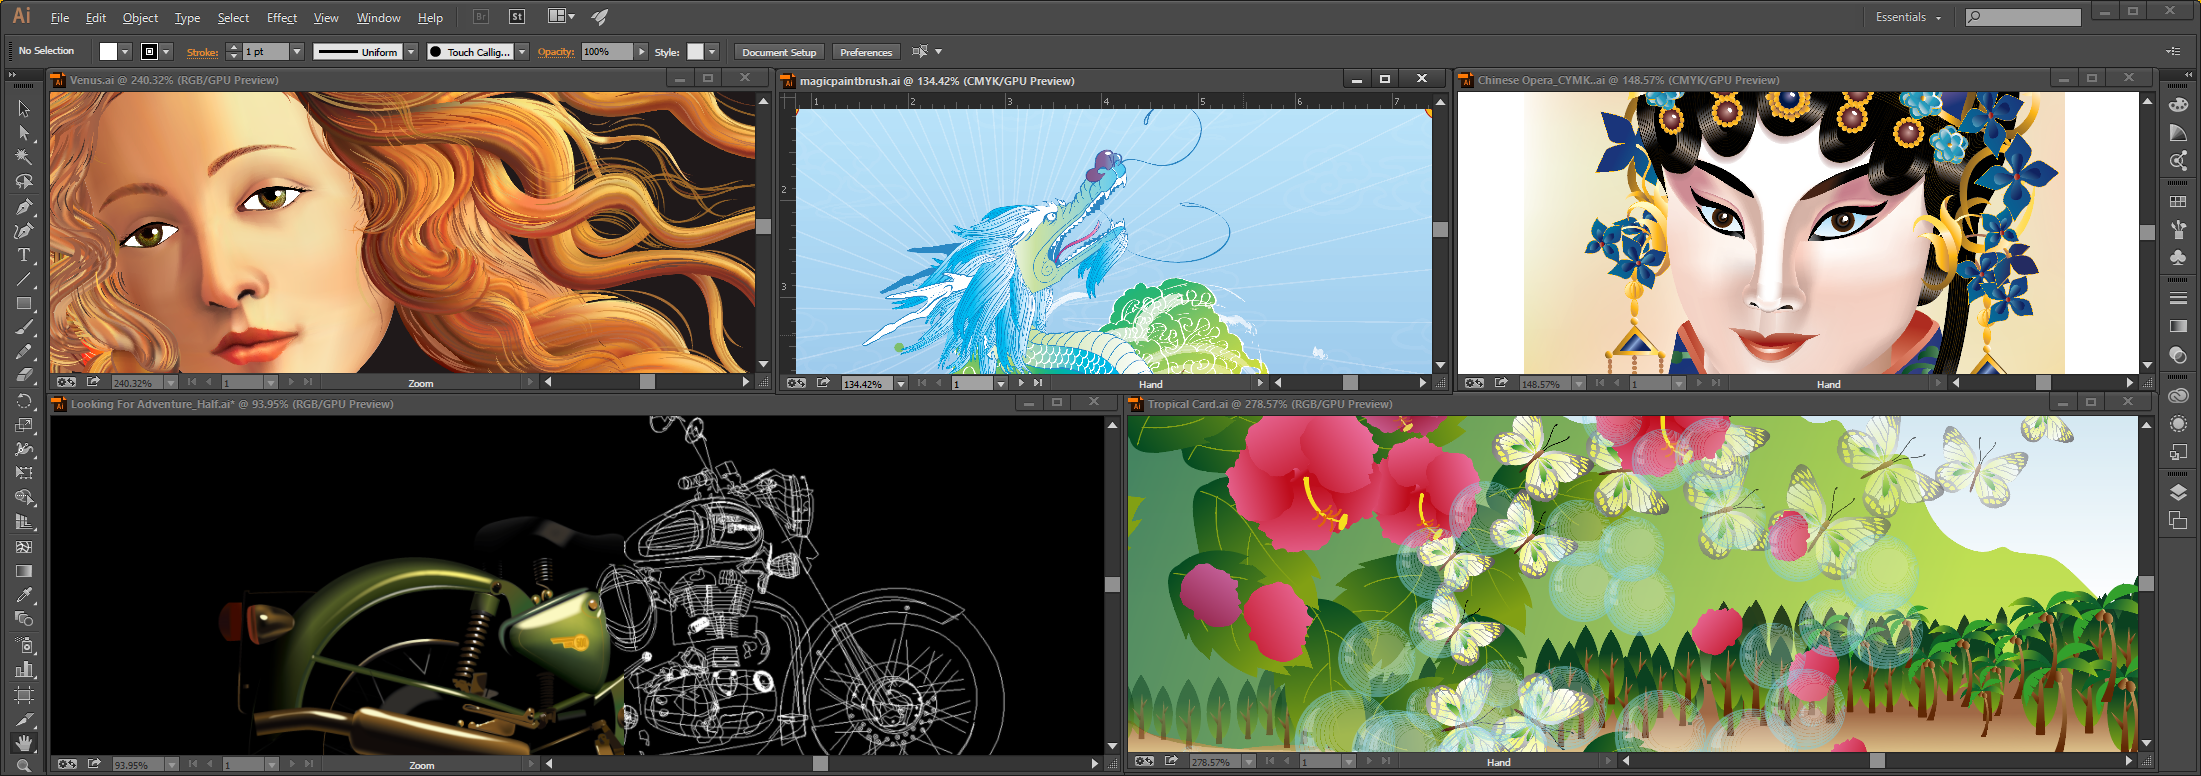
\includegraphics[width=\textwidth]{images/ai_teaser_Draft6.png}
  %\includegraphics[width=5in]{images/ai_teaser_Draft5.png}
  \caption{\label{fig:teaser} Five complex RGB and CMYK documents GPU-rendered by \IllustratorCC/; all rendered with ``GPU Preview'' enabled.}
}

\maketitle

% !TEX root = illustrator_submission.tex

\begin{abstract}

%Designers and artists worldwide rely on \AdobeIllustrator/ to edit vector graphics content.
We describe our successful initiative to accelerate
Adobe
\Illustrator/ with the graphics hardware pipeline of modern GPUs.
Relying on  OpenGL 4.4 plus recent OpenGL extensions for
advanced blend modes and first-class GPU-accelerated path rendering, we
accelerate the \AdobeGraphicsModel/ (\AGM/) layer responsible for rendering
sophisticated \Illustrator/ scenes.  \Illustrator/ documents render in
either an RGB or CMYK color mode.  While GPUs are designed and optimized
for RGB rendering, we orchestrate OpenGL rendering of vector content
in the proper CMYK color space and accommodate the 5+ color components
required.  We support both non-isolated and isolated transparency groups, knockout,
patterns, and arbitrary path clipping.  We harness GPU
tessellation to shade paths smoothly with gradient meshes.  We do all this
and render complex \Illustrator/ scenes 2 to 6x faster than CPU rendering
at Full HD resolutions; and 5 to 16x faster at Ultra HD resolutions.

\end{abstract}



\begin{CRcatlist}
  \CRcat{I.3.4}{Computer Graphics}{Graphics Utilities}{Graphics Editors};
  %\CRcat{I.3.4}{Computer Graphics}{Graphics Utilities}{Picture Description languages};
\end{CRcatlist}

\keywordlist

% !TEX root = illustrator_submission.tex

\section{Introduction}
\label{sec:intro}

%% The ``\copyrightspace'' command must be the first command after the 
%% start of the first section of the body of your paper. It ensures the
%% copyright space is left at the bottom of the first column on the first
%% page of your paper.

\copyrightspace

Designers and artists worldwide rely on \AdobeIllustrator/
to design and edit
resolution-independent 2D artwork and typographic content.
\Illustrator/ was Adobe's very first application when released over 27 years ago.

Prior to our work, no version utilized graphics hardware to accelerate \Illustrator/'s rendering.
All rendering was performed entirely by the CPU.
This situation is in stark contrast to the now ubiquitous GPU-acceleration of 3D graphics rendering
in Computer-Aided Design, Animation, and Modeling applications.  So while other graphical content creation applications
readily benefit from the past 15 years of improvements in GPU functionality and performance, \Illustrator/
could neither benefit from nor scale with the tremendous strides in GPU functionality and performance.
Our work remedies this situation as Figure~\ref{fig:teaser} shows.

The starting point for our work is OpenGL 4.4 \cite{GL44spec}
and the GPU-accelerated ``stencil, then cover'' path rendering functionality described in \cite{KilgardBolz2012}.
While the \NVpr/ OpenGL extension \cite{NVpr}
provides very fast and resolution-independent rendering of first-class path objects just as we need, \Illustrator/'s
rendering model requires much more than merely rendering paths.  
We had to develop our own strategies to handle features of
\Illustrator/ that, while dependent on path rendering, require considerably more sophisticated orchestration of the GPU.
We focus on the GPU-based techniques we developed and productized to accomplish
full GPU-acceleration of \Illustrator/.

Adobe
originally developed \Illustrator/ as a vector graphics editor for PostScript \cite{PLRM} which implements the
imaging model described by \cite{Warnock:1982:DIG:800064.801297}.
\Illustrator/ today depends on the Portable Document Format (PDF) standard for its underlying rendering capabilities
as described by the ISO 32000 standard \cite{PDF-Spec}.  The evolution of PostScript to PDF introduced a number
of sophisticated graphics capabilities for dealing with printer color spaces, compositing, and photorealistic artistic shading.
These capabilities developed in parallel with but isolated from
contemporaneous hardware-oriented improvements in interactive 3D graphics.
PDF and \Illustrator/ incorporated features and solutions relevant to
the print industry such as subtractive color spaces, typography, and
rasterization of 2D spline-based content targeting print engines with
extremely high pixel density.  However GPU hardware designers essentially
ignored such concerns---instead focusing on interactive 3D graphics.

For example, GPUs specialize at rendering RGB colors---typically with alpha, so RGBA---for
display on emissive RGB monitors.  Indeed the framebuffer, texture, and memory subsystems of GPUs are 
tailored specifically for handling 4-component RGBA colors.
However \Illustrator/ users target printed color output and expect accurate color reproduction
so the default document color mode in \Illustrator/ is CMYK, a color space intended for printed content.
\Illustrator/ also does support RGB documents but CMYK matters more to professional users.

Rather than just 4 color components as GPUs are designed to handle well,
CMYK involves at least 5 components (the process ink colors {\em cyan}, {\em magenta},
{\em yellow}, and {\em black} + alpha) and then additional {\em spot} colors assigned to specific custom inks.
Simply converting CMYK colors to RGB and rendering in an RGB color space is not the same as rendering into
a proper CMYK color space as Figure~\ref{fig:cmyk-vs-rgb-emulation} shows.
Among the differences, CMYK is a subtractive color space while RGB is an additive color
space so color arithmetic such as blending must account for this difference.
When a GPU's data paths are so specialized for processing RGBA values with exactly
4 components, handling 5 or more components in a manner consistent with PDF
requirements and at reasonable efficiency requires novel treatment.

\subsection{Motivation}

Our work to GPU-accelerate \Illustrator/ has the obvious goal of improving
the rendering speed and interactivity to improve user productivity.  \Illustrator/
documents can become extremely complex and so poor rendering performance
can frustrate a designer's creativity.

We also considered display technology trends, particularly increasing screen resolutions and
pixel densities.  So-called {\em 4K} resolutions such as Ultra HD at 3840x2160
are particularly interesting to us.
CPU performance scaling for rendering in \Illustrator/ has clearly not
been adequate to keep up with the increasing number of pixels needing to be rendered.
Recent 5K Ultra HD (5120x2880) displays make this more pressing.

%%%We also observe how the proliferation of non-PC devices are creating a multitude of pixel resolutions
%%%to which to deploy resolution-independent 2D content.

While our focus has been fully accelerating {\em existing} features of the PDF rendering model, we
anticipate our transition of \Illustrator/'s rendering to the GPU allows us to accelerate graphics
operations, known as {\em effects} in \Illustrator/, that are handled ``above'' the PDF rendering model currently.
Gaussian blurs and image warps are obvious examples of effects the GPU could significantly accelerate.
\ifdefined\NOSHOW
Prior to \Illustrator/'s GPU-acceleration, processing effects with the
GPU was simply untenable because the inputs and outputs of effects reside in system
memory where they are not efficiently accessible to the GPU.
\fi

% When all Illustrator rendering occurs on the GPU, effect acceleration becomes possible.

\subsection{Contributions and Outline}
\label{sec:contributions}

Our key contributions are:
\begin{itemize}

\item Novel repurposing of the GPU's multiple RGBA render buffers for {\em NChannel} color space rendering of CMYK process colors and additional spot colors with full blending support.

\item GPU algorithms to composite both isolated and non-isolated transparency groups properly.

\item Tessellating gradient meshes to shade paths via GPU hardware tessellation.

\item Harnessing ``stencil, then cover'' path rendering to support arbitrary path clipping, pattern shading, and knockout groups.

\item Rendering complex vector scenes with the GPU many times faster than comparable multi-core CPU rendering.

\end{itemize}
These contributions are broadly applicable beyond \Illustrator/ and benefit
any GPU-accelerated software system that
utilizes PDF, SVG, or similar printing, web, or vector graphics standards.
We anticipate web browsers, other 2D digital content creation applications,
document previewers, and even printers will use our contributions
to accelerate existing standards for resolution-independent 2D vector graphics.

Furthermore we expect GPU-acceleration of \Illustrator/ to motivate graphics hardware architects
to focus on specific optimizations for this important rendering model.  Likewise research in GPU-based  techniques for vector
graphics becomes substantially easier to productize.

Section~\ref{sec:relatedwork} outlines relevant prior work.  Section~\ref{sec:background} provides useful background for \Illustrator/'s
software architecture relevant to rendering. 
Section~\ref{sec:blendmodes} discusses GPU support for blend modes, a prerequisite for our contributions.
Sections~\ref{sec:cmyk} to \ref{sec:shading} describe the primary techniques we developed
to GPU-accelerate Illustrator fully.  Section~\ref{sec:comparison} compares and contrasts our GPU-acceleration to Illustrator's existing CPU renderer.   Section~\ref{sec:performance} presents our performance improvements.  Section~\ref{sec:conclusion} concludes
with a call for standardization and discussion of future plans.

\subsection{Status}

The June 2014 release of \AdobeIllustratorCC/ first incorporated our
GPU-acceleration efforts.  Adobe reports over 3.4 million Creative
Cloud subscribers as of December 2014.  A substantial fraction of
these subscribers use \Illustrator/.
The complete
contributions we discuss are refinements beyond the initial release.
In particular, the 2015 version introduces CMYK
(Section~\ref{sec:cmyk}) and tessellation-based gradient meshes (Section
\ref{sec:gradient-meshes}).


% !TEX root = illustrator_submission.tex

\section{Related Work}
\label{sec:relatedwork}

The PDF specification \cite{PDF-Spec} describes in detail the rendering model \Illustrator/ implements.
Kilgard and Bolz \shortcite{KilgardBolz2012} provides a good review of GPU-acceleration approaches for path rendering
and is the crucial underlying functionality upon which our work relies.  

Our interest in rendering complex
vector graphics scenes is similar to the random-access vector texture approach of
\cite{Nehab:2008:RRG:1457515.1409088} and its refinement by \cite{Leben:Thesis:2010}.
However \Illustrator/'s raison d'\^{e}tre is arbitrary editing of vector graphics scenes in a very general
setting (permitting CMYK color spaces, blend modes, transparency groups, etc.) so the need to
re-encode the scene's vector texture whenever the scene is manipulated is unappealing.

Vector textures are also unappealing because we must support all of \Illustrator/'s rich feature set but
a vector texture scheme 
effectively centralizes support for the scene's entire rendering requirements.  This means
the fragment shader used to decode the vector texture approach
must be prepared to incorporate every possible vector graphics feature in the scene.
The advantage of random-access decoding when rendering from a vector texture, while interesting, is not particularly relevant
to \Illustrator/.

Recent work by \cite{GanEtAl14} has significantly advanced the vector texture approach by using CUDA
to implement massively-parallel vector graphics on the GPU
rather than the conventional graphics pipeline.
Section~\ref{sec:mpvg} compares their reported performance to ours so we defer more discussion until then.

\subsection{Alternative Vector Graphics Editors}

While there are many alternative path-based vector graphics editors, such as Inkscape \cite{kirsanov2009inkscape}
and CorelDRAW \cite{CorelDRAWbook},
no existing vector graphics editor significantly exploits graphics hardware
acceleration to the best of our knowledge.

While not a conventional path-based editor,
the Mischief application \cite{MischiefWebPage} for scalable drawing, sketching, and painting is GPU-accelerated.
Mischief takes an Adaptive Distance Field (ADF) approach
\cite{Frisken:2006:DDF:1185657.1185675}.  ADFs represent shape implicitly
rather than the explicit path-based approach used by \Illustrator/ and PDF
to represent shape. A hybridization of Mischief's implicit approach and our explicit approach may be possible
given the commonality of GPU-acceleration.

\subsection{Smooth Shading} 

The PDF standard provides several shading operators for continuous color. 
Linear and radial gradients are very familiar to 2D digital artists and are a standard way for
integrating continuous color into vector graphics content.  For example, the SVG standard \cite{SVG-Spec} supports
both linear and radial gradients.  Our GPU-acceleration efforts accelerate both linear and radial
gradients using straightforward cover shaders as described in \cite{KilgardBolz2012}.

\Illustrator/'s {\em gradient mesh} tool provides a way to shade paths using
a mesh of Coons patches to assign and edit continuous color within a path \cite{PDF-Spec,CoonsPaper}.
Skilled artists use gradient meshes to create editable photorealistic resolution-independent artwork,
often sampling colors for the mesh control points from photographs.
%Researchers have explored techniques to assist in the generation of
%gradient meshes \cite{Sun:2007:IVU:1276377.1276391,Lai:2009:ATG:1531326.1531391}.

A different approach to
assigning smooth color to vector graphics artwork called {\em diffusion curves} \cite{Orzan:2013:DCV:2483852.2483873,Sun:2012:DCT:2185520.2185570,Ilbery:2013:BDC:2508363.2508426} relies on
partitioning 2D space with vector-based primitives and letting color naturally ``diffuse'' through the
scene to a steady-state that respects the partitions.  The color diffusion process is computationally intensive and
well-suited for the massively parallel nature of the GPU.  Our immediate interest is accelerating
\Illustrator/'s existing gradient mesh functionality though we anticipate our transition to the GPU
facilitates the adoption of more intuitive gradient methods otherwise too expensive for the CPU.


% !TEX root = illustrator_submission.tex

\section{Illustrator Rendering Architecture}
\label{sec:background}

\begin{figure}[tb]
  \center{
     %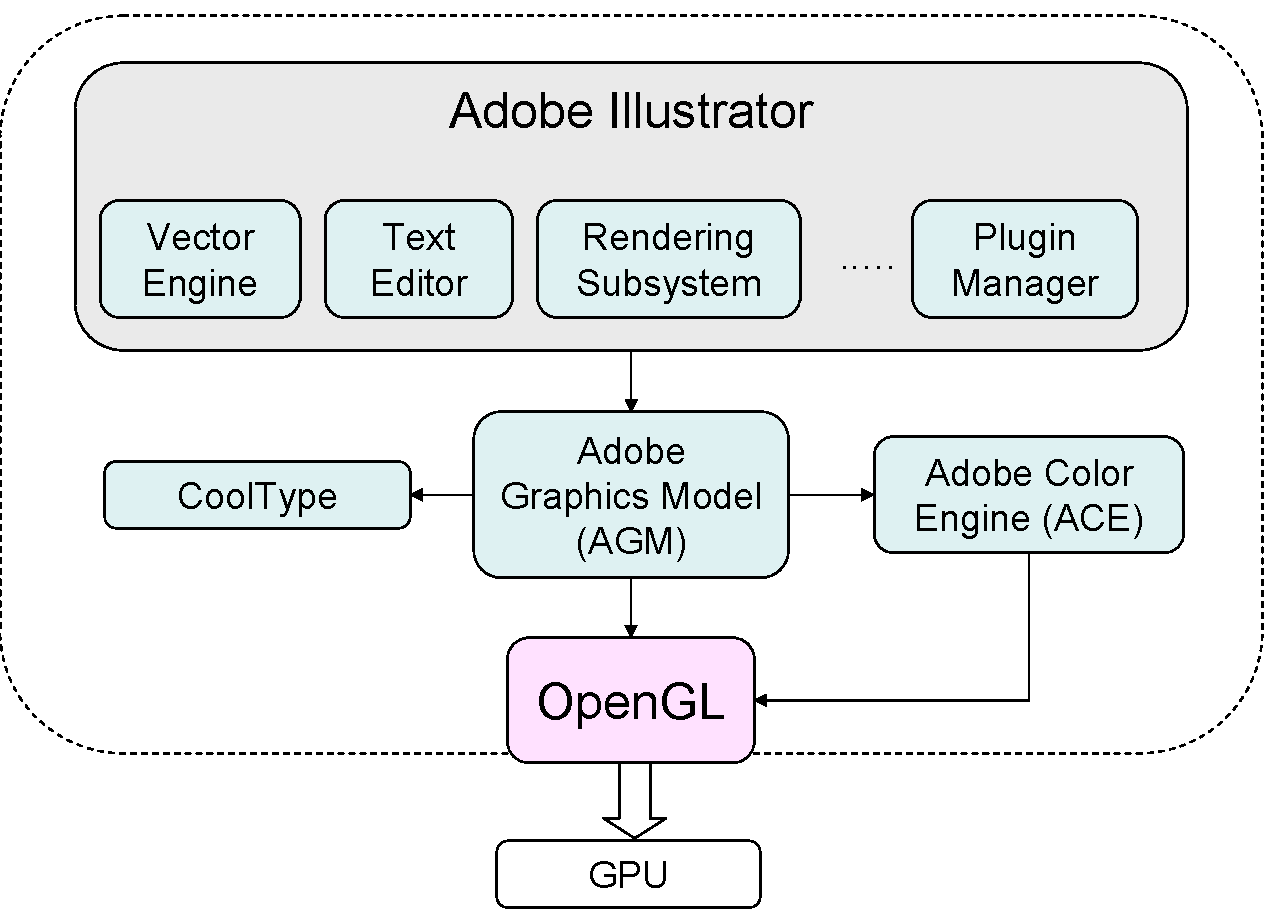
\includegraphics[width=2.6in]{images/IllustratorBlockDiagram.pdf}
     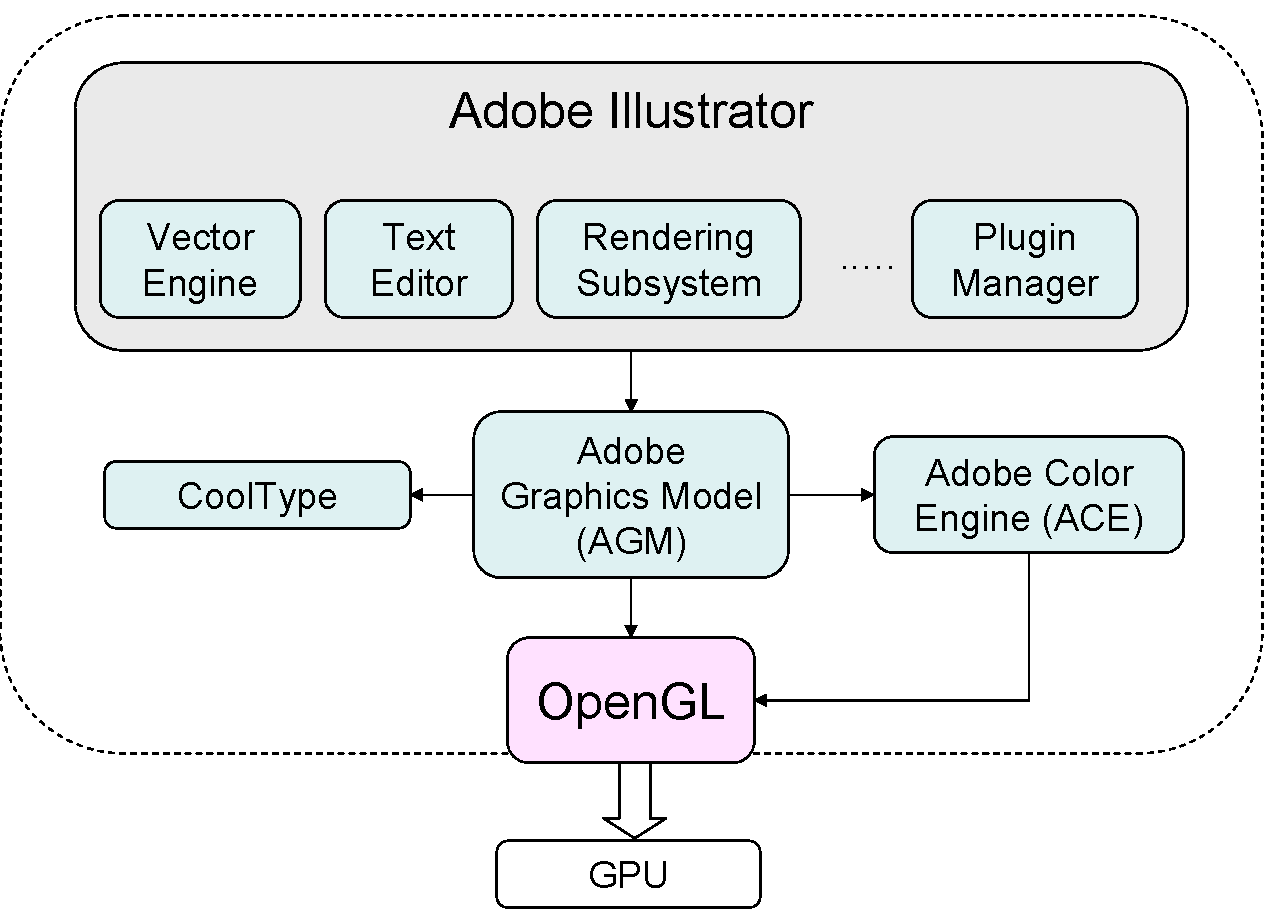
\includegraphics[width=\columnwidth]{images/IllustratorBlockDiagram.pdf}
  }
  \caption{Organization of major rendering-related modules within \Illustrator/.}
  \label{fig:illustrator-block-diagram}
\end{figure}

The software architecture of \Illustrator/ comprises several interoperable modules shown in
Figure~\ref{fig:illustrator-block-diagram} that have evolved over decades.

\ifdefined\NOSHOW
These include:
\begin{itemize}
\item
Vector Engine for creating and manipulating content with cubic B\'{e}zier splines. 
\item
Text Editor which implements rich text editing features and font handling.
\item
Plugin Manager for dynamically extending functionality (e.g. 3D support, cartography, etc.) using pluggable components (including third party plugins).
\end{itemize}
\fi

Our paper focuses on the Rendering Subsystem
for rasterizing vector content at arbitrary resolutions
so any further detail
about other modules is beyond our scope.  Despite the
complexity of \Illustrator/ overall, our GPU-acceleration effort required modifying
only the Rendering Subsystem and its subcomponents.
	
\AnIllustrator/ {\em artwork} (analogous to a 3D scene graph but for vector graphics) comprises
multiple art objects (B\'{e}zier-based path, text, image, mesh, etc.), each
attributed with a collection of {\em appearances} (fill and stroke with solid color,
pattern, gradient, etc.) and {\em effects} on these appearances (blur, feather,
shadow, etc.). When stacked in Z-order, these art objects interact with
each other to produce rich content. This interaction (or composition)
is based in the PDF specification. \Illustrator/ also provides several
high level primitives that are not supported directly in the PDF
specification but are reducible to PDF constructs. An example is an
\Illustrator/ path with both fill and stroke applied, which is reduced
to two paths---a path with stroke placed on top of a path with
fill. Figure~\ref{fig:artwork-layer} shows another example where an art
object with {\em OffsetPath} and {\em OuterGlow} effects is reduced to a group
comprising three compound paths and an image.

\begin{figure}[tb]
  \center{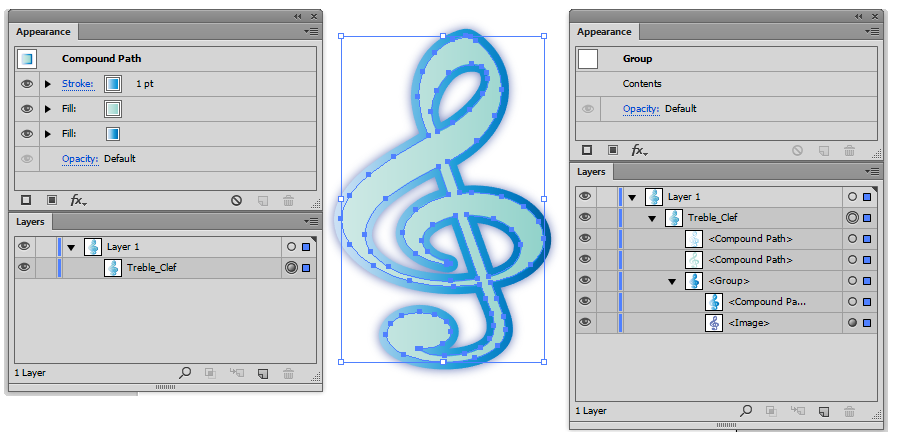
\includegraphics[width=3.3in]{images/artwork_layer.png}}
  \caption{How high-level artwork with effects applied (left) for a treble clef scene (center) reduces to a tree of PDF constructs (right).}
  \label{fig:artwork-layer}
\end{figure}

In service to the Rendering Subsystem, the {\em \AdobeGraphicsModel/} (\AGM/) layer
provides a pipeline for rendering PDF compliant artwork using the CPU
and now---with our work---the GPU.
For managing the color output by a target device, \AGM/ uses
\AdobeColorEngine/ (ACE) which implements color conversions
between different profiles on the GPU using GLSL shaders.
ACE profile management handles many different target devices (monitor, mobile devices, printer, etc.)
to ensure accurate color reproduction.
Font support is
implemented via \CoolType/ that provides programming interfaces for retrieving
font and glyph information (including glyph outlines) from system
fonts.
Figure~\ref{fig:illustrator-block-diagram} shows the relationship of
\AGM/, ACE, CoolType and OpenGL.
Our acceleration effort focused essentially entirely
on accelerating \AGM/ so we rely on higher level graphics primitives to be
reduced to the PDF rendering model.


% !TEX root = illustrator_submission.tex

\section{Blend Modes}
\label{sec:blendmodes}

%Illustrator 9 first introduced and supported the PDF 1.4 transparency model \cite{TransparencyInPDF}.
%While intricate in its details, the basic
%model composites two colors, corresponding to an object ({\em source}) and backdrop ({\em destination}),
%to generate a single color result (typically the {\em new destination}) based on a palette of
%{\em blend mode} functions quantifying how the two input colors interact.

%\subsection{GPU Fixed-function Blending Insufficient}

\ifdefined\NOSHOW
\begin{figure}[tb]
  \center{\includegraphics[width=3.1in]{images/fixedfunction_blending.pdf}}
  \caption{\label{fig:fixedfunction-blending}
  Conventional fixed-function blending; just RGB data flow is shown but scalar alpha data path is similar..}
\end{figure}
\fi

%In the interest of hardware simplicity and performance,
%GPU hardware blending is generally implemented as a fixed-function unit capable of performing
%simple blending functions constructed with rudimentary math operations (i.e. multiplies, adds, min/max)
%%and minimal control logic.
%% as shown in Figure~\ref{fig:fixedfunction-blending}.
%The hardware blending functionality in OpenGL is sufficient to implement all the
%blend functions introduced by the compositing algebra of \cite{Porter:1984:CDI:800031.808606}.

\begin{figure}[tb]
  \center{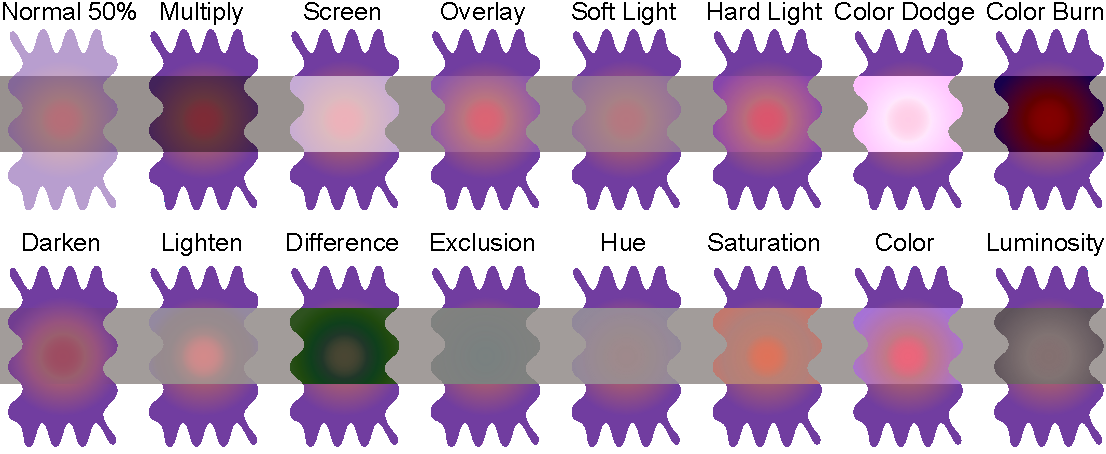
\includegraphics[width=3.3in]{images/blendmode_example.pdf}}
  \caption{\label{fig:blendmode-example} Example of all sixteen blend modes showing the interaction between a blob with an opacity gradient interacting with an overlapping rectangle with 90\% opacity.}
\end{figure}

Illustrator version 9 introduced a palette of sixteen blend modes.
These blend modes were subsequently incorporated into
the PDF standard's transparency model \cite{TransparencyInPDF}.

\subsection{GPU Blend Mode Support}

Of these modes
only two ({\em Normal} and {\em Screen}) are sufficiently simple that
they can be implemented with conventional OpenGL fixed-function blending.
Several of the advanced PDF
blend modes require intermediate numeric range exceeding the clamped [0,1] range
used in fixed-function GPU blending.
Some of the modes require simple ``if/then/else'' conditions, division, and square root operations.
To a hardware designer or anyone else first encountering these modes, they may seem {\em ad hoc} and  arbitrary,
but {\em HardLight}, {\em ColorDodge}, and the rest are firmly established in the vocabulary and training of digital artists \cite{HiddenPowerOfBlendModes}.  Figure~\ref{fig:blendmode-example} demonstrates their various effects.

\ifdefined\NOSHOW
Blending is the last step in the traditional GPU rendering pipeline and necessarily operates
at the {\em per-color sample} rasterization rate
(rather than {\em per-pixel} rate of multisample fragment shading)
and {\em after} stencil testing.
These are both important considerations
for Illustrator because blend modes and shading each specified independently and our
antialiased \NVpr/ usage relies on both 8x multisampling and stencil testing.
Even if blend modes
were extremely rare in real content,
the consequence of implementing a fallback to handle
the unsupported blend modes is very expensive, both in terms of poor performance and implementation
complexity.  \Illustrators/ 8x multisampling means {\em per-sample shading}
could run as slow as \nicefrac{1}{8}
%one-eighth
speed.
In practice, blend modes are sufficiently common in Illustrator artwork
to need efficient handling.
\fi

\ifdefined\NOSHOW
In anticipation of Adobe's requirements for blend mode support to GPU-accelerate
Illustrator,
%\footnote{Though blend modes are no longer limited to PDF and \Illustrator/.
%Flash \cite{SWF-File-Format}, SVG, and other
%compositing standards also incorporate blend modes (though the details
%vary).}
NVIDIA developed the OpenGL \NVbea/ extension \cite{NVbeaSpec}
and implemented its {\em coherent} flavor in their Tegra K1 and Maxwell GPUs.
Khronos subsequently standardized a multi-vendor subset \KHRbea/ \cite{KHRbeaSpec} to provide
the specific blend modes \Illustrator/, PDF, and SVG \cite{SVG-Compositing-Spec} require.
Either extension is sufficient for \Illustrators/ blending needs.

For NVIDIA GPUs that pre-date
this blend mode hardware functionality, the {\em incoherent} flavor of \NVbea/ and \KHRbea/ are
advertised and implemented through shader epilogues managed automatically
by the driver.  There is one explicit limitation of the non-coherent flavor: explicit {\em blend barrier} commands
must be used to ensure properly ordered blending.  However a special
exception is made for \NVpr/'s rendering operations because ``stencil,
then cover'' path rendering naturally lends itself to proper ordering.
For \Illustrator/, this means the same blend equation advanced programming interface
works on both older and newer NVIDIA GPUs without needing explicit blend barriers.
\fi

In anticipation of Adobe's requirements for blend mode support, NVIDIA
developed the OpenGL \NVbea/ extension \cite{NVbeaSpec} for advanced blending.  It
provides
all the blend modes needed by Illustrator, PDF, and SVG \cite{SVG-Compositing-Spec}.
The first-class {\em coherent} form of the extension
is implemented via hardware support in Tegra K1 and Maxwell
GPUs.
For older GPUs without hardware support for the coherent form,
the advanced blending functionality is exposed
through an {\em incoherent} form of the extension.
For the incoherent form, drivers 
are expected to implement the advanced blending as
a driver-generated epilogue to the application's fragment shader.
The incoherent form
requires the application to use
blend barrier commands to ensure proper blend ordering
to guard against read-modify-write hazards.
A special exception is made for \NVpr/
operations, since ``stencil, then cover'' path rendering naturally lends
itself to proper blending.

Khronos subsequently standardized OpenGL advanced blending functionality with the \KHRbea/
\cite{KHRbeaSpec} extension, also with coherent and incoherent forms.
AGM uses either OpenGL extension as available.

%\begin{figure}[tb]
%  \center{\includegraphics[width=2.8in]{images/iterated_blend.pdf}}
%  \caption{\label{fig:iterated-blend} Iterated blend hardware unit (right) as alternative to fixed-function blending (left).
%  %(see Figure~\ref{fig:fixedfunction-blending}).
%  }
%\end{figure}

\ifdefined\NOSHOW
\subsection{Alternative Hardware Approaches}
\label{sec:blendalternatives}

Recent hardware advances provide alternatives to introducing specific
blend modes.  Intel's {\tt INTEL\_fragment\_shader\_ordering}
\cite{INTELfsoSpec} (also supported by AMD GPUs) and NVIDIA's
{\tt NV\_fragment\_shader\_interlock} \cite{NVfsiSpec} provide
similer-but-different ``safely ordered'' mechanisms for the fragment
shaders to access the multisample framebuffer contents and perform arbitrary shader
computations within that shader.  If one tries to avoid the high cost of per-sample shading, 
the performance challenge for efficient per-pixel shading is the shader must perform
the blend mode math on each rasterized color sample within the pixel (times 8 in our case) but only
for color samples that pass the stencil test (relevant if color sample writes are done directly
by the shader rather than with conventional blending of the shader's color output).

While the viability of our GPU-acceleration effort and our contributions
(Section \ref{sec:contributions}) require some mechanism to handle all
PDF blend modes---and consideration of these alternatives is worthy of
investigation---their evaluation is outside the scope of the present
work.
\fi

\subsection{Premultiplied Alpha}
\label{sec:premultiplied}

One point of interest for GPU blending is how colors are represented.  Colors stored in GPU framebuffers and
textures must to be stored in pre-multiplied alpha form \cite{PreMultAlpha} for correct blending (including blend modes)
and texture filtering.  In contrast, the CPU-based AGM renderer stores color values with non-premultiplied alpha
consistent with the PDF specification.


% !TEX root = illustrator_submission.tex

\section{CMYK Support}
\label{sec:cmyk}

\Illustrator/ artwork is typically authored in the CMYK color space---optionally with spot color components---to
best facilitate high-quality color printing.
\Illustrator/ uses \AGM/ to render CMYK documents to a true CMYK framebuffer.
This means the color components in the rendered framebuffer
correspond to actual CMYK process colors plus any spot colors so blending and other color math
operates on and maintains the components independently.

What the artists sees ``on screen'' when editing a CMYK document is a color conversion from CMYK plus any spot colors
to RGB.  Importantly this conversion happens on the {\em final} CMYK rendering result; the conversion may even emulate the
specific color profile of a particular print device using ACE.
Converting CMYK rendering results to a print device's CMYK
color profile results in better color fidelity and gives an artist better access to the printer's full color gamut
including spot color inks.  Importantly spot color components stay segregated from process colors.

While it is possible to force the conversion of all CMYK color inputs to RGB and render in the GPU's conventional
RGB mode, Figure~\ref{fig:cmyk-vs-rgb-emulation} shows
the inadequacy of rendering CMYK content with this approach; notice the obvious color shifts.

\begin{figure}[tb]
  \center{\includegraphics[width=3.3in]{images/cmyk_vs_rgb_emulation.pdf}}
  \caption{\label{fig:cmyk-vs-rgb-emulation} An artistic CMYK \Illustrator/ document (left, correct) properly rendered
in its intended CMYK color space; na\"{\i}ve RGB rendering (right-side, wrong) of same scene by converting all inputs to RGB .  Magnified portion show obvious gross color shifts.}
\end{figure}

Now we explain our approach to orchestrate CMYK rendering with multiple RGBA color buffers.
The technique we present works not just for \Illustrator/ but any GPU application that requires
CMYK rendering semantics.

There are two problems we must address:
\begin{enumerate}
\item CMYK is a subtractive color space so conventional GPU blending modes do not blend appropriately for CMYK.
\item At a minimum, CMYK rendering needs 5 framebuffer components---plus additional components for any spot colors.
\end{enumerate}

\subsection{CMYK Blend Modes and Color Math}
\label{sec:cmykblend}

Adobe's technical note introducing transparency to PDF \cite{TransparencyInPDF} explains how blending
in a subtractive color space requires special handling:
\begin{quote}
\small
When performing blending
operations in subtractive color spaces, we assume that the color component values are complemented before the blend mode function is applied and that the results of the function are then complemented before being used. By
complemented we mean that a color component value $c$ is replaced with $1 - c$. 
\end{quote}
An example helps appreciate why:  Consider a black ink at 90\% of its full application (so a dark black).  Now
consider how to get 40\% of the apparent brightness of that ink.  Intuitively 40\% brightness should be an
even darker black.
Na\"{\i}vely multiplying 0.9 by 0.4, as appropriate for additive color
components, is 36\% but less black ink is clearly incorrect.
Adjusting the blending math for the subtractive nature of black ink,
$1-((1-0.9)\times(1-0.4))$ = 94\% results in more black ink and the darker black we intuitively expect.

\begin{figure}[tb]
  \center{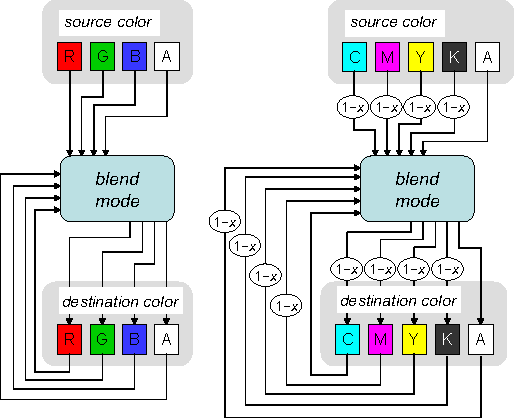
\includegraphics[width=2.9in]{images/rgba_vs_cmyk_blending.pdf}}
  \caption{\label{fig:rgba-vs-cmyk-blending} RGBA blending works normally (left); CMYK's subtractive color space must complement colors components on input and output of blending (right).}
\end{figure}

Figure~\ref{fig:rgba-vs-cmyk-blending} illustrates how RGB and CMYK
color values must be treated for a blend mode to operate correctly.
Conventional fixed-function GPU blending lacks the ability to complement
inputs and outputs to fixed-function blending.

The blend mode extensions described in Section~\ref{sec:blendmodes}
assume an additive color space.  Na\"{i}vely
adapting these blend modes to operate
correctly for a subtractive color space such as CMYK would mean adding
a complement to each input color component and, likewise, a complement
to each output color component.  We avoid the na\"{i}ve approach because
\begin{enumerate}

\item Additive blend modes avoid input \& output color component
complements so involve fewer operation
and are therefore more efficient.

This is particularly important for legacy hardware that predates
hardware blend mode support.
For such hardware, performing additional input \& output complements for
CMYK rendering would force expensive shader emulation
even for the default {\em Normal} blend mode that otherwise
can be performed with fast standard hardware blending.

\item Not just blending math
requires this adjustment---{\em all} color math such as in a shader or texture filtering must follow the rule.

\end{enumerate}
Our solution stores CMYK color components always in complemented form on the GPU.
Figure~\ref{fig:cmyk-gpu-blending} illustrates this approach.  Incoming CMYK colors, no matter what the source, must be
complemented.  Alpha values are {\em not} complemented and simply stored normally as alpha is always additive.

\begin{figure}[tb]
  \center{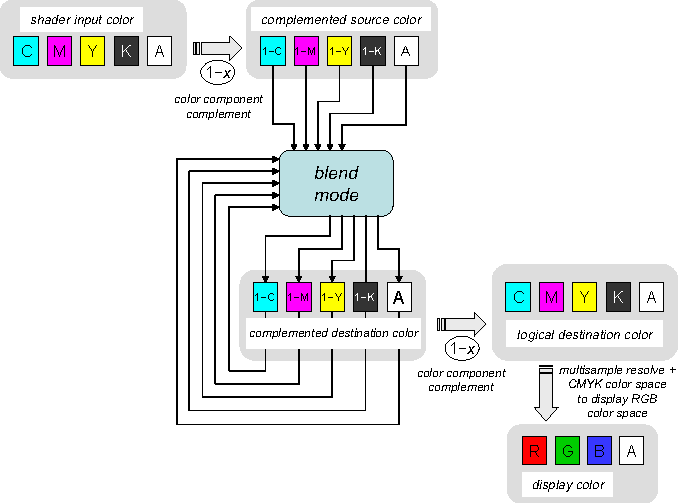
\includegraphics[width=\columnwidth]{images/cmyk_gpu_blending.pdf}}
  \caption{\label{fig:cmyk-gpu-blending} Conventional GPU blending works for CMYK when color components (but not alpha) are stored as complemented values.}
\end{figure}

The implications of this are far reaching and demand rigorous consistency.
Any CMYK or RGB color inputs must be converted to
complemented CMYK. 
For example, when color channels are logically ``cleared to zero,'' that really means clearing to one (but alpha
components still clear to zero).
By storing complemented CMYK colors in the framebuffer {\em and} in textures,
existing hardware texture accesses to such resources including texture filtering operate properly.
Likewise programmable
shaders are simpler and faster by skipping the requirement to complement input and output colors
by performing color math
on complemented subtractive color values.

Importantly our solution means the blend modes provided by the blend
equation advanced extensions operate in subtractive CMYK color mode
with exactly the same blending math as additive RGB color mode.

Only when rendered results are ready to be displayed or read back to
system memory should the complemented color components be reversed to uncomplemented CMYK.
Often color profiles are applied when displaying
or reading back rendering results so the necessary complement can be folded into a more complex conversion
thereby avoiding an explicit complement.  The bottom right two steps in Figure~\ref{fig:cmyk-gpu-blending} show this.

\subsection{Representing an NChannel Framebuffer on a GPU}
\label{sec:representing-cmyk}

When we speak of \Illustrator/'s CMYK color mode,
we mean a subtractive color spaces supporting the 4 standard print
process colors (CMYK), alpha, and possibly some fixed number of spot colors.  PDF supports
a variety of color spaces with different properties and degrees of sophistication.
The most general of these is the {\em NChannel}
color space so we use the term NChannel to refer to a general multi-component color space.

\subsubsection{Multiple Color Buffers}
\label{sec:multiplebuffers}

GPUs lack native support for color buffer configurations with more than 4 components.
However modern GPUs also support multiple (typically eight) color buffers to which a single
fragment shader can output a distinct RGBA value to each color buffer.  Each color buffer
is independently blended with its respective RGBA output value.

% UNINTERESTING
% Modern GPUs support {\em separate} fixed-function blend functions and equations
% on the RGB and A components of each 4-component RGBA color buffer.  The relevant point being that
% the fourth component, alpha, can be configured for blend math different than the other three (RGB).
% Indeed blend modes composite the alpha component different from the color components, hence
% this specialized behavior.

\begin{figure}[tb]
  \center{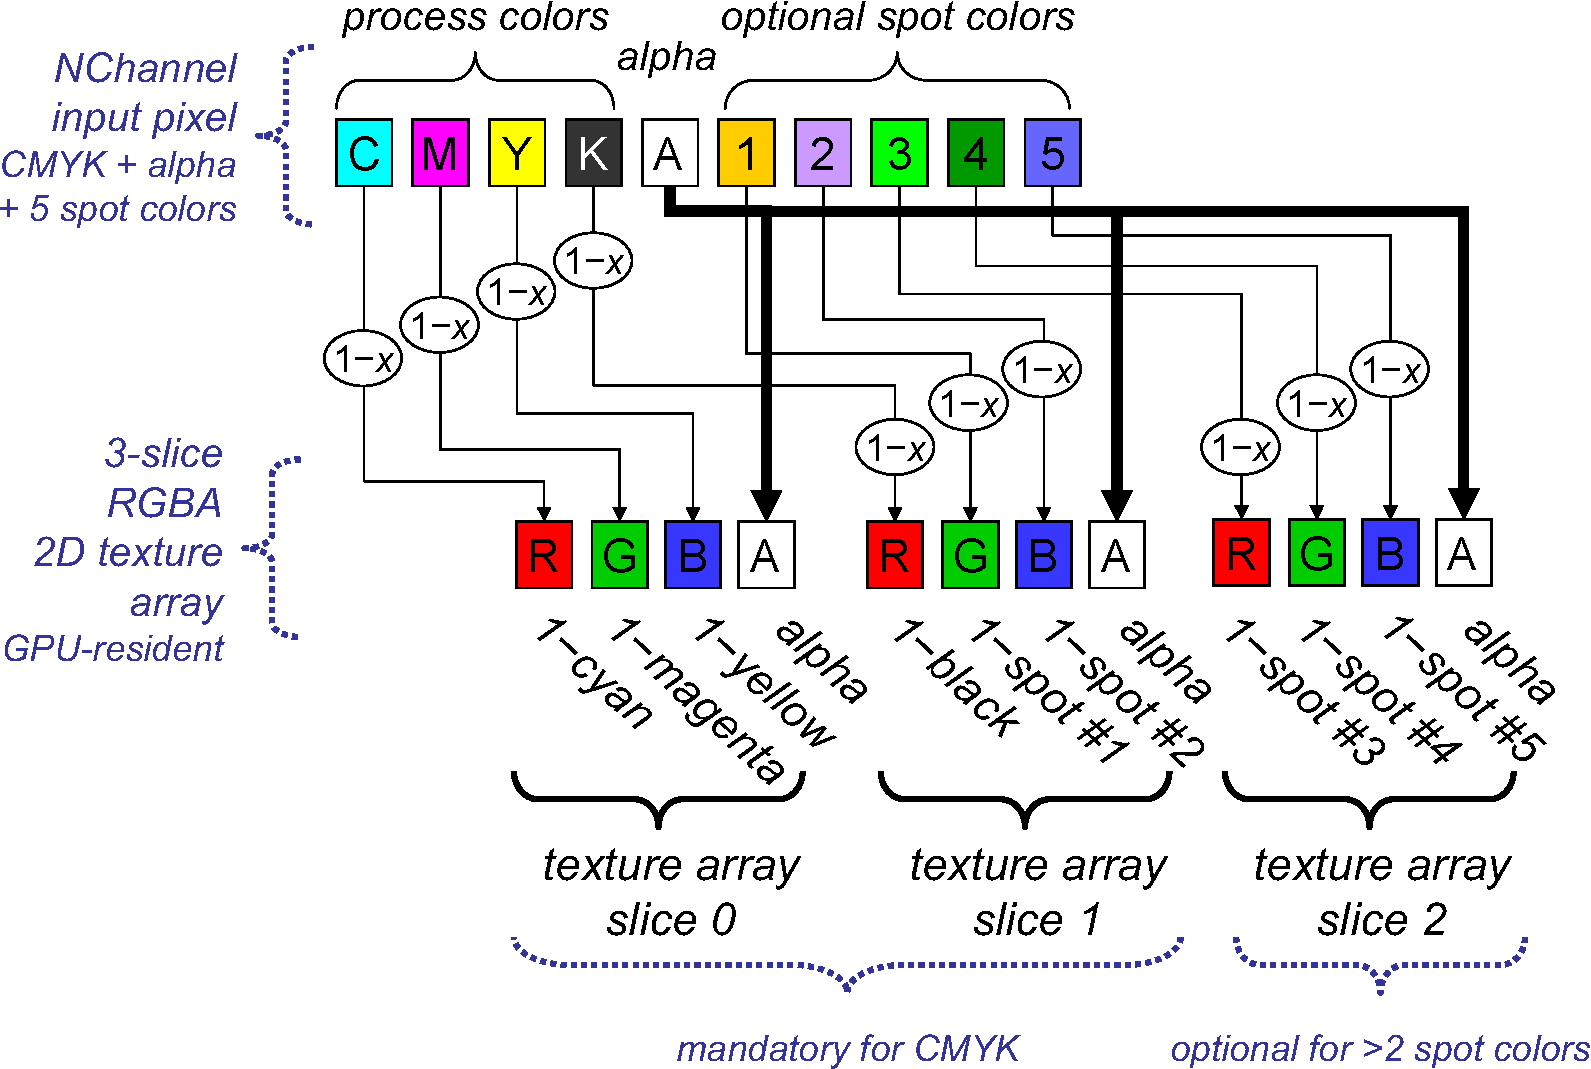
\includegraphics[width=3.3in]{images/cmyk_to_gpu_representation.pdf}}
  \caption{\label{fig:cmyk-to-rgba} How NChannel color components in a CMYK color space with spot colors are converted to a GPU-resident version.}
\end{figure}

We orchestrate multiple color buffers to ``construct'' an NChannel framebuffer with CMYKA components plus any
additional spot color components.
Figure~\ref{fig:cmyk-to-rgba} illustrates how we take a CMYKA input color with five spot color components
and convert this 10-component vector into a GPU-amenable representation by spanning three RGBA color buffers.
We can span additional color buffers to support more spot colors but we always require at least two
RGBA color buffers for CMYKA.

Figure~\ref{fig:cmyk-to-rgba} shows we {\em replicate} the alpha (A) component in the alpha of each RGBA color buffer.
This is done because blend mode equations for color values require access to the alpha component.  As GPU blending performs
each color buffer blending operation separately, replication of alpha ensures every three color components
of the NChannel color spanning multiple RGBA buffers has an accessible alpha value.  We deliberately replicate
alpha this way and ensure all alpha blending is identically configured so the alpha values of
each RGBA color buffer for any specific color sample maintain the {\em same} alpha value.
This invariant must be maintained for correct operation.

\subsubsection{Memory Requirements}
\label{sec:memory}

Our approach wastes some storage.
Every additional RGBA buffer adds an
additional replicated alpha component.  We also waste storage if the actual CMYK color mode configuration
has fewer spot colors than our multiple RGBA color buffers provide.  For example, CMYKA with zero spot
colors means the G and B components of the second color buffer are wasted---assuming R is used to store K.
The unfortunate implication is that a document in CMYK color mode without spot colors requires double
the framebuffer memory as an RGBA document.

This waste is substantial when coupled with \Illustrator/'s reliance on 8x multisampling for antialiasing.
When also accounting for the stencil buffer requirements, representing CMYK at 8x on today's GPUs requires 96 bytes
of storage per pixel.\footnote{96 bytes = $8 \times$ ( 4 bytes for depth-stencil + 8 bytes for CMYKA)}  
Each gigabyte of memory roughly corresponds to
representing 5.5 million CMYKA pixels this way.
The waste is ameliorated by the enormous memory capacity and bandwidth of modern GPUs.
Graphics boards with 12 gigabytes of memory are available today and capacities are sure to increase.

We anticipate GPU hardware innovations
will provide less wasteful memory organizations in future GPUs. In the interim
when the memory burden is just too taxing, settling for 4x antialiasing quality
easily halves the memory requirements at the cost of diminished rendering quality.

\subsubsection{Fragment Shader and Blending Implementation Details}
\label{sec:tweaks}

Once we have orchestrated multiple color buffers to store NChannel color values, our fragment shaders
must adapt to outputting color values appropriately.  This means making sure alpha is replicated in each
output color buffer alpha component and each process and spot color
is routed to its appropriate component in the correct color buffer.  

GPU color blending should be configured the same across all the framebuffer components.

One irksome detail:  The blend equation advanced extensions are restricted to operate only where outputting to the
first color buffer and requiring all other color buffers disabled (otherwise an OpenGL error is generated; this
reflects a hardware limitation).  We workaround this limitation with multiple ``cover'' steps.
We ``stencil'' the path once and then perform the path rendering ``cover''
operation repeatedly, once for each color buffer
(binding each color buffer in turn as the first and only color buffer)
and reset the stencil values only on the last color buffer.
Our fragment shader must be aware in this case which logical color buffer it is outputting in each repeated ``cover'' step.
While expensive, we only require this workaround for blend modes (typically the less common
ones) that do not correspond to fixed-function GPU blending---so importantly not the {\em Normal} mode.

\subsubsection{Reading an NChannel Framebuffer from a Shader}

\Illustrator/ occasionally needs to read a framebuffer from a shader.
(see Section~\ref{sec:non-isolated-groups} for an example).
To enable efficient texture lookup, we
organize the multiple color buffers
used to represent an NChannel
buffer
as layers
of a multisample 2D {\em texture array} ({\tt sampler2DMSArray} in GLSL
shaders).  A 2D texture array
is a single OpenGL texture object with a fixed format, width, height, and number of layers. 
When
multisampled, the number of samples is also fixed.
The {\tt texelFetch} command in a shader fetches an RGBA
floating-point vector sample from a given 2D location, layer index, and sample index (effectively a 4-dimensional array access).
Multiple {\tt texel\-Fetch} fetches, one to each layer, are necessary
from the fragment shader to read all the components of a pixel in an
NChannel framebuffer.

The \ARBtms/ extension \cite{TextureMultisample} introduced support for
multisampled 2D texture arrays with OpenGL 3.2 mandating the functionality.
Among the advantages of a multisampled 2D texture array is all the layers belong to a single texture memory allocation
making the layers faster to bind as a unit and managed as a single large memory allocation.
The OpenGL command {\tt glFramebuffer\-Texture\-Layer} allows
each layer of the texture array to be attached to different color buffer
of single framebuffer object.


% !TEX root = illustrator_submission.tex

\section{Transparency Groups}
\label{sec:transparency-groups}

In Section~\ref{sec:blendmodes}'s discussion of blend modes, we assumed objects are simply blended in object stacking
order with blend modes directing the blending.
The PDF~1.4 transparency model becomes more intricate when graphics objects are grouped.
Transparency groups, or simply {\em groups}, allow a sequence of consecutive objects to be
collected together and composited
to produce a single color and opacity at each color sample.  Groups facilitate independent sub-scenes
to be composited together.  Artists also use groups to combine objects for artistic effects such
as darkening or lightening regions.  Groups can be nested within other groups to form a tree of groups.
When a group is reduced to a single color and opacity, the group itself has a blend mode and a per-group opacity 
used to composite the group with its backdrop.
Transparency groups are a distinct concept from other mechanisms to
group objects such as groups formed to manage hierarchical
transforms or inherited properties.

\subsection{Isolated versus Non-isolated Groups}
\label{sec:transparency-groups}

Groups can be either {\em non-isolated} (\Illustrator/'s default for a new group) or
{\em isolated}.\footnote{The SVG Compositing specification \cite{SVG-Compositing-Spec}
has the same concept but calls the property {\em enable-background} where
the value {\em accumulate} matches non-isolated and {\em new} matches isolated.}
This distinction is
which backdrop is used when compositing objects in the group.  With a non-isolated group, the backdrop is ``inherited''
from whatever has already been rendered prior in the object stacking order.  This allows
a group to interact with the prior objects ``beneath'' the group.  With an isolated group, the backdrop is
fully transparent so it has neither color, shape, nor opacity.
This is sometimes called rendering ``on glass'' because there is really
nothing for the group to interact with when the group itself is rendered.  The group's rendering is---as the name implies---isolated.

Both modes are useful in their proper context.  Non-isolated groups make sense when rendering a group expects to
interact with the artwork beneath it.  For example, a non-isolated group makes sense when
an artist wants to use a blend mode such as {\em ColorDodge}
or {\em ColorBurn} where painting with black or white respectively preserves the backdrop color.  Compositing
a source object using these blend modes with an isolated group would not make much sense because the 
initial backdrop is fully transparent so there is no color to preserve.

Isolated groups are more appropriate when the group is considered
a fully resolved piece of artwork you simply want to composite into the scene.  For example, a piece of
vector clip art consisting of objects rendered with the {\em Normal} blend mode and
that otherwise has no blending relationship with what's been rendered so far.

\subsubsection{Framebuffer Management for Groups}
\label{sec:isolated-groups}

Of the two types of groups, non-isolated is the more expensive to implement.  Both types of groups
conceptually create a transient framebuffer necessary to resolve the color, shape, and opacity of the group.
We call this a {\em framebuffer instance} and we implement the group's framebuffer instance with an OpenGL framebuffer object
(FBO) distinct
from the current framebuffer instance.  Allocating and discarding transient FBOs during rendering
is inefficient so we manage a set of framebuffer resources sufficient to handle the scene's maximum
non-trivial group nesting.  Each framebuffer instance needs independent color buffer storage---and CMYK needs multiple
color buffers as Section~\ref{sec:representing-cmyk} discusses.  However all the framebuffer instances can share
a single stencil buffer.  This stencil sharing is useful for maintaining the clip path nesting and conserving GPU
memory usage.  Because each FBO used to manage transient layers is preallocated and may be used to render a
group positioned
arbitrarily 
within the scene's viewport, each FBO is maintained at the same dimensions as the base framebuffer instance (typically sized to match the maximum window-space view size) and expects to share a single stencil buffer.

We speak of {\em non-trivial} groups because in common cases where every blend mode within a group is {\em Normal}
and the group opacity is fully opaque (and other uncommon group features such as knock-out are inactive),
rendering a group to its own framebuffer instance is functionally identical
to simply rendering the group's objects in sequence into the current framebuffer instance. Recognizing trivial
groups and not instantiating a framebuffer instance for them is an important performance optimization.

But in cases when a non-trivial group is present, we carefully orchestrate rendering to a framebuffer
instance and when the group is resolved, compositing the resolved framebuffer layer for the group back into
the previously current framebuffer layer.  Because groups can be nested to form a tree, this process is
conceptually recursive but practically limited by the scene's maximum non-trivial group nesting.

From this point on, our discussion deals with non-trivial groups.

\subsubsection{Implementing Non-isolated Groups}
\label{sec:non-isolated-groups}

\begin{figure}[tb]
  \center{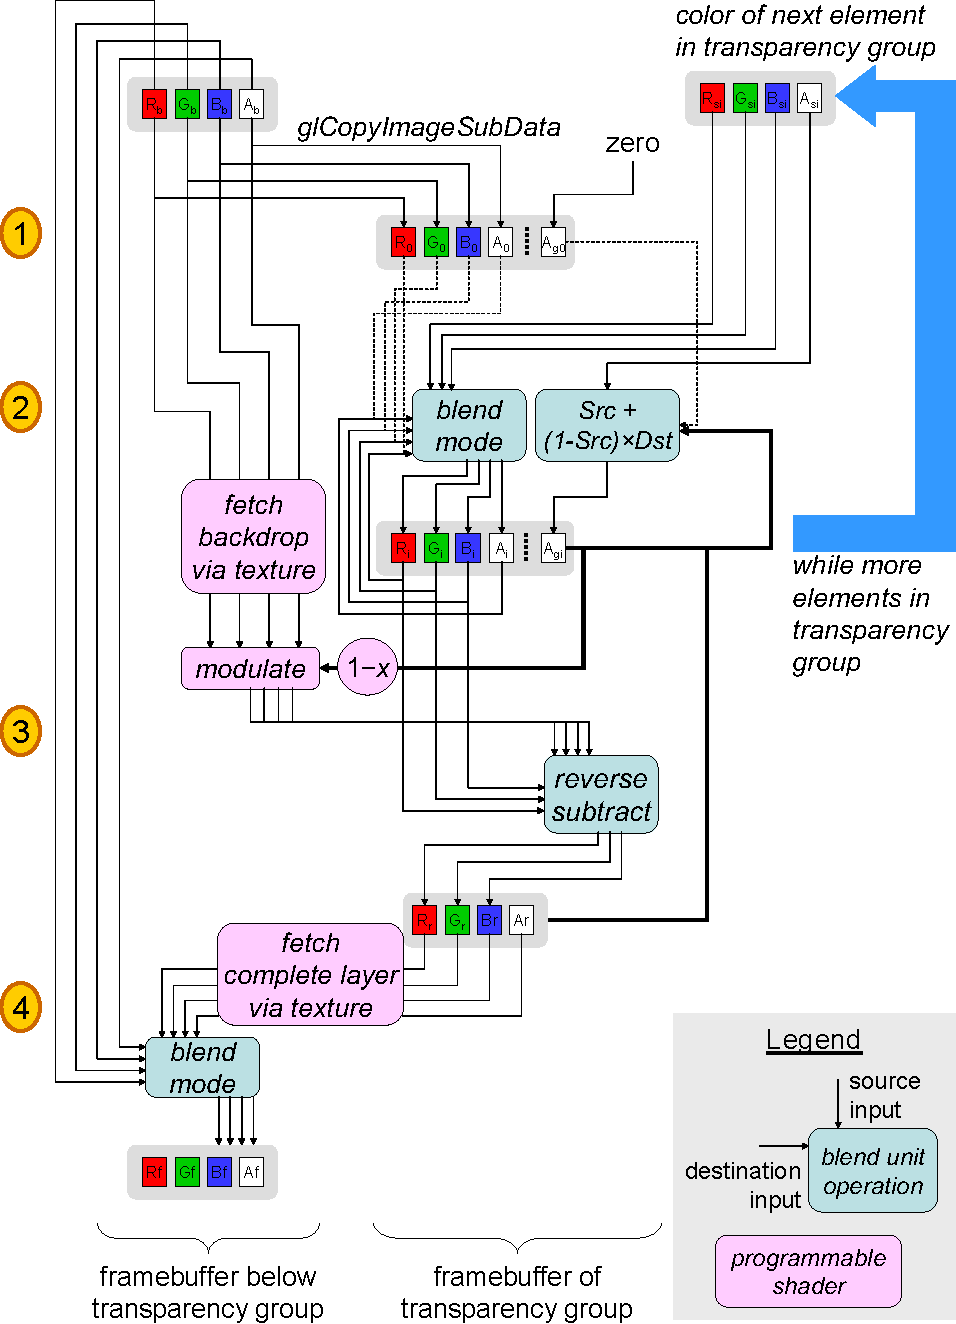
\includegraphics[width=\columnwidth]{images/non_isolated_group.pdf}}
  \caption{\label{fig:non-isolated-group} Four steps in rendering a non-isolated group with the GPU.}
\end{figure}

Figure~\ref{fig:non-isolated-group} illustrates the steps to process and resolve a non-isolated group
assuming an RGB color space.
Numbered circles down the figure's left side indicate the steps 1, 2, 3, and 4 to be discussed in turn.

{\bf Step 1:}
Establishing a non-isolated group requires copying the backdrop from the current framebuffer instance
to the group's transient FBO's color buffer(s).  OpenGL's {\tt glCopyImageSubData} command \cite{CopyImageSpec} copies
a rectangular region of texel color values
from one color buffer's underlying texture object to another.  When the color buffers are multisampled, the command
copies each pixel's individual color samples.  In the worst case, we may have to copy the entire
color buffer contents but often we can bound the window-space bounding box for the objects within the
group (including any nested groups).  CMYK has multiple color buffers configured as layers of
a texture array but a single {\tt glCopyImageSubData} command can copy all the texture array layers.

An additional single-component (red) color buffer is also required for the FBO to maintain the non-isolated group's
{\em group alpha} and labeled $A_{g0}$  and $A_{gi}$ in the Figure~\ref{fig:non-isolated-group}.
A scissored {\tt glClear} command must clear the {\em group alpha} color buffer to zero
The motivation for {\em group alpha} will be more clear in Step~3.

{\bf Step 2:}
Each element of the group must be rendered in object stacking order.  Any object that is a non-trivial
group requires that nested group to be rendered and resolved.  In such cases, the resolved color and opacity
of the nested group is composited using the group element's blend mode and group opacity into this
framebuffer instance.  Elements of trivial groups can simply be rendered in sequence.

During step 2, in addition to compositing group elements into the RGB color buffer (or buffers for CMYK),
the {\em group opacity} buffer is configured for PDF's {\em Normal} blending (implemented in OpenGL with
the {\tt GL\_ONE,GL\_ONE\_MINUS\_\-SRC\_ALPHA} blend function).  The fragment shader is responsible to output
the alpha of each group element to this color buffer.  The {\em group alpha} buffer is used to keep
a distinct running accumulation of alpha but starting from zero from the alpha component(s) in the
other (4-component) color buffers.

{\bf Step 3:} 
Before the resolved color in a non-isolated group can be composited back to the prior
framebuffer instance from before processing the group, we must ``subtract out'' the backdrop color and alpha
used to initialize the group's framebuffer instance by {\tt glCopyImageSubData}.  Otherwise when the
resolved color of the group is composited back into the prior framebuffer instance (Step~4), the
prior framebuffer instance's color and alpha would be accounted for twice.

The PDF specification computes the resolved result of a non-isolated transparency group with the equations:
\begin{align}
\label{eq:straight-non-isolated-color}
C & = C_n + (C_{n} - C_{0}) \times \left( \frac{\alpha_{0}}{\alpha_{gn}} - \alpha_{0} \right) \\
%
\label{eq:straight-non-isolated-alpha}
\alpha & = \alpha_{gn}
\end{align}
where $C$ is the resolved group color, $C_{n}$ is the final color in the framebuffer instance after all $n$ group
elements are composited, $C_{0}$ and $\alpha_{0}$ are the backdrop color and alpha respectively
from the prior framebuffer instance, and $\alpha_{gn}$ is the final {\em group alpha} from the
single-channel color buffer after all $n$ group elements are composited.

This equation is written with non-premultiplied alpha but the GPU represents colors in pre-multiplied alpha form.
Combining the Equations~\ref{eq:straight-non-isolated-color} and \ref{eq:straight-non-isolated-alpha} to find $\alpha C$ simplifies to:
\begin{equation}
\label{eq:premult-non-isolated}
\alpha C = \alpha_{n} C_{n} \left( \frac{\alpha_{gn} + (1-\alpha_{gn}) \alpha_{0}}{\alpha_{n}} \right) - (1-\alpha_{gn}) \alpha_{0} C_{0}
\end{equation}
We recognize the fractional expression in Equation~\ref{eq:premult-non-isolated} reduces to unity
because  $\alpha_{gn} + (1-\alpha_{gn}) \alpha_{0}$ is $\alpha_{n}$ because 
the alpha composition of the final {\em group alpha} with the backdrop alpha $\alpha_{0}$ is simply $\alpha_{n}$
as alpha compositing is associative.

So Equation~\ref{eq:premult-non-isolated} simplifies to:
\begin{equation}
\label{eq:simple-premult-non-isolated}
\alpha C = \alpha_{n} C_{n} - (1-\alpha_{gn}) \alpha_{0} C_{0}
\end{equation}
Equation~\ref{eq:simple-premult-non-isolated} can be realized in OpenGL by rendering a conservative window-space rectangle
matching the rectangle used for the earlier {\tt glCopyImageSubData} command with this subtractive blend
\begin{verbatim}
  glBlendEquation(GL_FUNC_REVERSE_SUBTRACT);
  glBlendFunc(GL_ONE, GL_ONE);
\end{verbatim}
and a per-color sample fragment shader that outputs the product of fetching color values from the prior framebuffer
instance to get $C_{0}$ and one minus the texel $\alpha_{gn}$ fetched from the single-component {\em group
alpha} color buffer.

{\bf Step 4:} 
Lastly composite the resolved group color $\alpha C$ and opacity $\alpha$ back to the prior framebuffer instance by
rendering
with per-sample shading
another conservative window-space rectangle, here applying the blend mode for the group.
The logical Steps 3 and 4
can be advantageously combined into a single rendering pass.

\subsubsection{Implementing Isolated Groups}
\label{sec:isolated-groups}

Isolated groups are easier.
The isolated group rendering process follows the same general structure as shown in
Figure~\ref{fig:non-isolated-group} except Step 1 simply clears the group's framebuffer instance color buffer(s)
to fully transparent.  For RGB, this is clearing the color buffer to zero.  For CMYK, this is clearing the
RGB components to one and alpha component to zero.  No {\tt glCopyImageSubData} command is necessary.

Since an isolated group does not copy the backdrop from the prior framebuffer instance,
there is also no need to ``subtract out'' that backdrop in Step 3 so this step can be skipped.

Steps~2 and 4 operate in the same manner as for non-isolated groups.

\subsection{Knockout}
\label{sec:knockout}

By default, groups composite the elements of the group in their stacking
order and use the prior element's rendering result as their backdrop.
A group marked for knockout, known as a {\em knockout group}, always
uses the group's initial backdrop.  One common use of knock-out is
rendering semi-opaque annotations where the annotations may overlap but
double-blending of annotations is undesirable so only the last rendered annotation at
any given pixel should blend with the prior framebuffer instance (the
backdrop).

``Stencil, then cover'' path rendering provides an efficient way to
implement knockout by rendering the elements of the group in reverse
stacking order.  Blend normally during the ``cover'' step but mark every
updated stencil sample by setting an upper bit in the stencil buffer
for each updated color sample.  Then have further rendering by other
elements in the knockout group fail the stencil test if the stencil sample
value's upper bit is set.  This ensures color samples are only updated
and blended by the last element in the group's stacking order to cover
the color sample.  When all the group's elements have been rendered,
draw a conservative covering rectangle to unmark the stencil values so
normal ``stencil, then cover'' rendering can proceed.

Note that this
%{\em Caveat:} This
approach will not work if any of the immediate
elements of the knockout group are non-isolated-groups.
This uncommon case requires the non-isolated group element to use the
backdrop of prior group elements in the stacking order which the reverse
order will not have rendered so an explicit and involved knockout approach
is required.

% TOO LONG
%\subsection{Additional Transparency Features}
%
%Additional features of the PDF transparency model (soft masks, {\em
%alpha-is-shape}, page groups, and overprint) must also be GPU-accelerated
%and are mentioned here for completeness but are beyond the scope of this
%presentation due to space constraints and their relative unimportance
%compared to the other features discussed here.



% !TEX root = illustrator_submission.tex

\section{Shading}
\label{sec:shading}

\Illustrator/ supports constant color, linear gradients, radial gradients, and raster shading.
These straightforward shading modes are performed by ``cover'' fragment shaders
much as described by \cite{KilgardBolz2012} with short shaders.  The shaders must be tweaked
to support outputting to NChannel framebuffers but are otherwise not particularly noteworthy.
PDF's support for patterns and gradient meshes however present more interesting shading challenges.

\subsection{Patterns}
\label{sec:patterns}

A {\em pattern} consists of a small graphical figure called a pattern cell,
which is replicated at fixed horizontal and vertical intervals to
fill an area.  This process is called {\em tiling} the area.  The pattern cell
comprises graphical elements (such as paths, text, and images), may
be non-rectangular in shape, and the spacing of tiles can differ from
the dimensions of the cell itself.  To draw a pattern, the pattern cell
is drawn as many times as necessary to fill the given area.  We accomplish
this in one of two methods:
\begin{enumerate}

\item If a pattern object contains a non-isolated group with a blend
mode, the contents of a pattern cell are drawn at each step, clipped to
the tile area.

\item Otherwise, the contents of the pattern cell are drawn once into a
separate texture (which is of the same size as pattern cell), and this
texture is copied at each tile location.

\end{enumerate}

The actual process of clipping to a tile is the same method described by \cite{KilgardBolz2012}
to clip to an arbitrary path.

\subsection{Gradient Meshes} 
\label{sec:gradient-meshes}

The PDF specification provide several mesh-based shading techniques for vector objects:
\begin{itemize}
\item Free-form and lattice-form smooth shaded triangle meshes,
\item Coons patch \cite{CoonsPaper} meshes, and
\item Tensor-product patch meshes.
\end{itemize}

Triangle meshes are fairly straightforward as the GPU is excellent at rendering smooth-shaded color triangles.
The only caveats are we stencil test these triangles against the shaded object's stenciled region and use
a final ``cover'' step but with color writes disabled to make sure the stenciled region is reset.

\ifdefined\NOSHOW
\subsubsection{Triangle Meshes}

Shading by triangle meshes, whether free-form or lattice-form,
is straightforward to implement on the GPU.  The meshes are simply transformed and rasterized
as triangles with {\em smooth} (or PDF also supports {\em flat}) color interpolation.  Stencil testing against coverage generated by the ``stencil'' step
of ``stencil, then cover'' path rendering ensures the shading stays within the path object's stroked or filled coverage.
If the triangles in the mesh overlap, the last triangle to cover a color sample position decides that sample's color (no double blending allowed).  The most efficient way to accomplish this is rendering the mesh triangles in reverse and having
the stencil operation reset the stencil value when the stencil test passes and the sample's color is updated.  This
is more efficient since no color sample is updated by the triangle mesh more than once.  The mesh may not
cover all color samples within the region stenciled by the ``stencil'' step; to remedy this, a final ``cover'' step that simply resets
the stencil values to their neutral state (but not update the color buffer) when the stencil test passes
will ensure all 
stencil values within the path's stenciled region are reset.  Modern GPUs optimize for high stencil discard rates
so this extra ``cover'' step is inexpensive.
\fi

Patch meshes are more challenging than triangle meshes as edges of the patches are bicubic B\'{e}zier segments and the patch may fold over itself.  The na\"{\i}ve approach would expand the patch into a triangle mesh and render in the same manner as the shaded triangle meshes.  This has the disadvantage that a sufficiently tessellated triangle mesh to approximate each patch in a patch mesh (which might be hundreds of patches) is expensive for the CPU to generate and store.  Having to CPU-tessellate all the patches undermines the compactness and editability advantages of Coons patches.  Moreover the tessellated triangle meshes would be resolution-dependent so would not support fast zooming of the scene.

Fortunately modern GPUs support hardware tessellation units \cite{schaefer2014star}, but the application
of this hardware is primarily directed at depth-tested 3D models formed from tessellated patches.

We harness this same tessellation hardware to render PDF's Coons and tensor-product patch meshes, but we
identify some limitations of existing GPU hardware applied to our 2D tessellation task.
Hardware tessellation splits the process of rasterizing patches into
three programmable domains:
\begin{description}
\item[Vertex shading] facilitating the transformation of control points from object space to other spaces.
\item[Tessellation Control shading] accepting an array of control points (transformed by vertex shading) and outputting a fixed (possibly different) number
of control points, uniform patch values, and level-of-detail parameters to define a patch to evaluate.
\item[Tessellation Evaluation shading] evaluating the patch output from the tessellation control shader at a given ($u$,$v$) location within the patch as part of a mesh topology generated by fixed-function hardware.
\end{description}
At first glance, this hardware is readily amenable to tessellation of our 2D gradient mesh patches.
The vertex shader can transform vertices from object space into window-space.  The Tessellation Control Shader (TCS)
subsequently performs
a basis change from a Coons patch to a bicubic B\'{e}zier basis for ease of evaluation by the Tessellation Evaluation Shader (TES); the tensor-product patch is already a B\'{e}zier bicubic.  The TCS uses the window-space control point positions to compute
appropriate level-of-detail parameters to ensure every triangle in the tessellated topology is on the scale of about 1 to 2 pixels to minimize under or over tessellation.
The TES should evaluate the 2D position at its ($u$,$v$)
and interpolate a color based on color values assigned to the corner control points.  Still there are three
notable issues to address.

\paragraph{Resolving Mesh Overlap Render Order}

First GPU hardware tessellation does not guarantee the precise triangle
rasterization order for a patch.  This is justified because 1) 3D models are expected to be depth-tested to resolve hidden surface occlusion so there is no mandatory intra-patch triangle ordering (though the order is reasonably expected to
be deterministic); and 2) the hardware is more efficient if it can group vertices into triangles to maximize
vertex reuse.  However PDF mandates a particular order:
\begin{quote}
\small
Patches can sometimes appear to fold over on themselves---for example, if a boundary curve intersects itself. 
As the value of parameter $u$ or $v$ increases in parameter space, the location of the corresponding pixels in 
device space may change direction so that new pixels are mapped onto previous pixels already mapped. If 
more than one point ($u$, $v$) in parameter space is mapped to the same point in device space, the point selected 
shall be the one with the largest value of $v$. If multiple points have the same $v$, the one with the largest value of 
$u$ shall be selected. If one patch overlaps another, the patch that appears later in the data stream shall paint 
over the earlier one. 
\cite{PDF-Spec} \S 8.7.4.5.7
\end{quote}
This provides a tidy, well-defined order but does not match the actual hardware rendering order.
To resolve this, a combination of ($u$,$v$) and the current patch number
(indicated by {\tt gl\_InvocationID}) can be combined into a [0,1] value to use as a depth value.  For example:
\begin{verbatim}
  gl_Position.z = float(gl_InvocationID*65536
    + int(v*255)*256 + int(u*255))/ 16777215.0;
\end{verbatim}
Larger magnitude depth values are later in the rendering order.  When the gradient mesh is opaque such that
double blending is not a concern, depth buffering with a {\tt GL\_GREATER} depth buffer is sufficient to ensure
the gradient patch mesh ordering.  If that is not the case, a depth-only rendering pass to resolve the last
update to every color sample followed by a second {\tt GL\_EQUAL} depth function pass to assign interpolated color
and blend is necessary.

While we understand it is only the ordering of rasterized triangles within a patch that is implementation-dependent,
one or more patches may overlap a color sample so depth samples from different patches always compare with the latter patch in render order ``winning''.

Prior to rendering any set of patches, a depth clear to zero is necessary to reset the depth buffer.  This could
be done with a ``cover'' operation that simply zeros the depth buffer (without modifying other buffers) or with
a scissored depth buffer clear.
%{\tt glClear(GL\_DEPTH\_BUFFER\_BIT)}.

Once the render order issues are resolved, color shading is a matter of bicubic interpolation \cite{Sun:2007:IVU:1276377.1276391} in the TES.

This is a lot of complexity to match the PDF specification's patch rendering order.  Certainly if the hardware's
tessellation generator simply guaranteed an order consistent with the PDF specification, even at the cost of some
less optimal hardware efficiency, rendering PDF gradient meshes would be much more straightforward.

Another option is detecting via CPU preprocessing of the patch mesh whether or not actual mesh overlaps are present \cite{Randrianarivony04necessaryand}.
When not present, gradient mesh rendering could be much more straightforward and efficient.  In practice,
we know overlaps are rare in real gradient mesh content.

\ifdefined\NOSHOW

\paragraph{Assigning Colors to Patch Corners}

The Coons patch has twelve positional 2D control points while the tensor-product patch has sixteen.
But both Coons and tensor-product patches have just four colors, one for each patch corner.
In conventional triangle meshes, so-called {\em per-vertex} color attributes are assigned at every vertex position.
In the gradient mesh case, color values are assigned at just one-third or one-quarter the frequency of control points.

It is undesirable to assign colors for every control point vertex.  It both requires more static storage and
requires pulling vertex attributes for color that go unused.

\begin{figure}[tb]
  \center{\includegraphics[width=2.7in]{images/gradientmesh.pdf}}
  \caption{\label{fig:gradient-mesh}
Single gradient mesh patch showing 12 patch (x,y) control points of Coons patch
and 4 corner colors, where pairs of
control points provide the red-green and blue-alpha components.}
\end{figure}

Instead we segregate our vertex index values into two ranges, one for positions and one for colors with
a boundary index $b$.  Vertex index values below $b$ are positions and at or above are colors.  The vertex
shader transforms positions to window space while passing color components unmodified.  This allows
a single vertex attribute arrays indexing ($x$,$y$) values to interpret those values as either positions
or pairs of color components.  

Figure~\ref{fig:gradient-mesh} shows a Coons path with twenty control points
arriving in a TCS which treats the first twelve control points as 2D positions while the subsequent eight control
points make up the {\em red-green} and {\em blue-alpha} components of RGBA colors.  The advantage of this
approach is that positions and colors can be stored in a single buffer for efficient updating.  Extending
this to tensor-product patches or CMYK colors simply adds more control points for the additional data
and modify the TCS appropriately.
\fi

\paragraph{Coarse Level-of-detail Control}

Graphics hardware tessellation has a limited maximum level-of-detail for tessellation.  When the level-of-detail
is clamped to a hardware limit for tessellation, tessellation artifacts may arise.  We monitor the relative
size of tessellated patches such that their maximum level-of-detail does not grossly exceed the scale of two or three pixels
in window space.  If this happens, patches need to be subdivided manually to ensure the patch mesh
avoids objectionable tessellation artifacts.  Care is necessary to maintain a water-tight subdivided patch mesh.  This is done by ensuring exactly matching level-of-detail computations on mutual edges of adjacent patches.



 


\section{Comparing GPU versus CPU Rendering}
\label{sec:comparison}

%\begin{figure}[tb]
%  \center{
%     \includegraphics[width=2.5in]{images/gpu_performance_preferences.png}
%  }
%  \caption{Illustrator CC 2014 panel for GPU Performance.}
%  \label{fig:gpu-performance-preferences}
%\end{figure}

\begin{table*}
%\small
\centering
    \begin{tabular}{| E{1.4in} | L{2.3in} | L{2.6in} |} 
\hline
{\bf Capability} & {\bf CPU} & {\bf GPU} \\
\hline \hline

Per-component storage & 8-bit fixed-point components & 8-bit fixed-point components (same) \\
\hline

Color opacity representation & Non-premultiplied ({\em straight}) alpha & Premultiplied \S\ref{sec:premultiplied} \\
\hline

Per-pixel storage & One color value per pixel & Multisampling: 8 distinct (hardware compressed) colors per pixel + 8 stencil samples \S\ref{sec:memory} \\
\hline

CMYK representation & CMYK color components stored ``as is'' & Components stored complemented \S\ref{sec:cmykblend} \\
\hline

CMYK organization & N channels + alpha channel allocated as linear image in system memory & Multiple RGBA buffers, rendered as multiple render targets \S\ref{sec:multiplebuffers} \\
\hline

CMYK excess framebuffer \newline storage & None & Color components allocated in multiples of 3, with alpha duplicated for every 3 color components \S\ref{sec:multiplebuffers},\ref{sec:memory} \\
\hline

    \end{tabular}

\caption{Comparison of framebuffer storage and representation in CPU and GPU rendering modes for \Illustrator/.}
\label{table:framebuffer-compare}

\end{table*}

\begin{table*}
%\small
\centering
    \begin{tabular}{| E{1.4in} | L{2.3in} | L{2.6in} |} 
\hline
{\bf Capability} & {\bf CPU} & {\bf GPU} \\
\hline \hline

Rendering approach & Scan-line rasterization, professionally optimized & GPU ``stencil, then cover'' rendering via \NVpr/ \\
\hline

Rendering granularity & Cache of sub-image tiles for image reuse & Direct rendering to GPU framebuffer \\
\hline

Resolve to displayed color & Downsample of high resolution tile samples + apply color profile via CPU & Multisample downsample, then apply color profile via GLSL shader \\
\hline

Rendering implementation & C++ code directly manipulates pixels with CPU & CPU orchestrating OpenGL commands using GLSL shaders; pixel touching by GPU \\
\hline

Parallelism & Multi-core CPU rendering, divvying screen-space tiles among threads & GPU pipeline parallelism; NVIDIA dual-core OpenGL driver mode \\
\hline

Path control point transformation & CPU-based math & GPU-based vertex shading internal to \NVpr/ \\
\hline

Stroking & Conversion of stroked paths to fills & \NVpr/ stencils stroked paths directly---approximating cubic B\'{e}zier segments as a sequence of quadratic strokes \\
\hline

Antialiasing mechanism                  & Fractional coverage during scan-line rasterization & 8x multisampling \S\ref{sec:memory} \\
\hline

Blend modes & Optimized C++ with MMX and SSE intrinsics & Conventional GPU blending for {\em Normal} and {\em Screen}; \KHRbea/ for advanced PDF blend modes \S\ref{sec:blendmodes} \\
\hline

Non-isolated transparency group & Initialize (system memory) group framebuffer from lower layer contents; CPU render group with both non-isolated {\em and} isolated alpha; once group is rendered, composite from group framebuffer to lower layer after first subtracting out lower layer contents from group framebuffer & Allocate renderable GPU color texture(s) for layer {\em and} 1-component ``isolated alpha'' buffer cleared to zero; blit lower layer contents to new framebuffer object color contents; GPU render group with extra 1-component buffer accumulating isolated alpha; reverse subtract lower layer color from group color texture(s) based on isolated alpha; composite with blend mode color texture(s) for layer to lower layer framebuffer object \S\ref{sec:non-isolated-groups} \\
\hline

Isolated transparency group & Initialize group framebuffer (system memory) to clear; GPU render group with single alpha; once group is rendered, composite with blend mode from group framebuffer to lower layer & Allocate renderable GPU color texture(s) for layer; GPU render group; composite with blend mode color texture(s) for layer to lower layer framebuffer object \S\ref{sec:isolated-groups} \\
\hline

Knockout & Tagging pixels as done immediately once written in a knockout group & Reverse rendering of objects with the layer; unless combined with non-isolated group when depth buffering is used \S\ref{sec:knockout} \\
\hline

Path clipping & Concurrent scan-line rasterization of clip path & Stencil clip path with \NVpr/ into upper bits of the stencil buffer; then stencil draw path against stencil buffer upper bits \S\ref{sec:patterns} \\
\hline

Gradients & CPU shading code in C++ & GLSL fragment shaders with 1D texture for filtering and attribute generation by glPathTexGenNV \S\ref{sec:shading} \\
\hline

Gradient mesh implementation & CPU-based recursive mesh subdivision & Direct evaluation of 2D mesh vertex position \& color via GPU programmable tessellator, then hardware rasterization \S\ref{sec:gradient-meshes} \\
\hline

Implementation of Illustrator Effects (FX) & CPU-based effect plugin code processes layer image to make new image & Layer image must be read to CPU; CPU-based effect plugin code processes layer image to make new image; new image loaded as a texture and applied as image gradient \S\ref{sec:background} \\
\hline

    \end{tabular}

\caption{Comparison of rendering approaches in CPU and GPU rendering modes for \Illustrator/.}
\label{table:rendering-compare}

\end{table*}

Our contributions for GPU-acceleration are best understood in contrast
with Illustrator's pre-existing CPU rendering approach.
All but a cursory description of Illustrator's CPU rendering approach is beyond the scope of this paper.
Illustrator's CPU rendering closely follows the PDF standard \cite{PDF-Spec}.
AGM's CPU renderer
relies on a robust, expertly-tuned, but reasonably conventional active edge list algorithm
\cite{Foley:1990:CGP:83821}
for rasterizing arbitrary paths including B\'{e}zier segments \cite{TurnerFreeType2}.
Table \ref{table:framebuffer-compare} lists the differences between the CPU and GPU approaches in
organizing the framebuffer storage for rendering.
Table~\ref{table:rendering-compare} lists the ways rendering is different between the CPU and GPU approaches.

\ifdefined\NOSHOW
When the requirements for GPU-acceleration are met by the system, both CPU and GPU rendering are available.
%Figure~\ref{fig:gpu-performance-preferences} shows the ``GPU Performance'' panel.
The user can quickly toggle between the two rendering modes with a
keyboard shortcut (Ctrl-E) or the {\em View$\rightarrow$GPU Preview}
pulldown menu toggle option.  This ability to toggle the CPU versus GPU renderer
makes it easily for users (and Quality Assurance engineers)
to confirm they render essentially identical results---though not exactly pixel-for-pixel identical.
The tab above each artwork window ``GPU Preview'' when its contents are GPU rendered as shown in Figure~\ref{fig:teaser}.
\fi


% !TEX root = illustrator_submission.tex

\section{Performance}
\label{sec:performance}

We benchmarked our GPU-accelerated rendering mode against
\AGM/'s CPU-based renderer on six \Illustrator/
documents pictured in Figure \ref{fig:scenes}.  We selected these
scenes for their availability, artistic content, and complexity.
Table~\ref{table:scene-metrics} quantitatively summarizes each scene's
complexity.  We consider these scenes representative of the kind of
complex artwork we wish to encourage by making its authoring more
interactive.

\begin{table*}
%\small
\centering
    \begin{tabular}{| l | r | r | r | r | r | r | c |} 
\hline
      &       & 2D Control &  Clipping & Transparent  &           & Embedded & Native \\
Scene & Paths & Points     &  Masks    & Groups       & Gradients & Images & Color Space \\ \hline \hline

\hyperref[fig:bamboo]{WF\_BambooScene}	& 84,995 & 618,926 & 32,367 & 25,614 & 126 & 0 & CMYK	\\

\hyperref[fig:whale]{whale2}	& 14,403 & 481,928 & 14,333 & 14,313 & 0 & 0 & RGB	 \\

\hyperref[fig:archerfish]{ArcherFish}	& 11,214 & 	203,771 &  6,777 & 2,105 & 1,973 & 524 & RGB \\

\hyperref[fig:reef]{Tropical Reef}	&	1,041 & 6,698 & 0 & 0 & 291 & 0 & CMYK \\

\hyperref[fig:blue-mirror]{BlueMirror}	& 132,138 & 1,685,979	& 66,803 & 66,792 & 0 & 0 & RGB \\

%\hyperref[fig:beer-glass]{Beer-Glass}	&	13,151 & 141,075 & 6,579 & 6,572 & 0 & 0 & CMYK \\

%\hyperref[fig:carrot-tree]{Carrot Tree} 	& 13,998 & 129,529 & 3,672 & 3,362 & 194 & 3 & CMYK	\\

%\hyperref[fig:crowd]{Crowd (1)} 	&	93,599 & 2,627,594 & 41,941 & 41,880 & 0 & 1 & CMYK \\

\hyperref[fig:big-blend]{bigblend2} 	&	9,428 & 92,645 & 2,531 & 1,457 & 1,096 & 1 & CMYK \\

    \hline
    \end{tabular}

\caption{Scene complexity metrics.}
\label{table:scene-metrics}

\end{table*}

\begin{figure}
\centering
\subfigure[WF\_BambooScene.ai]{
   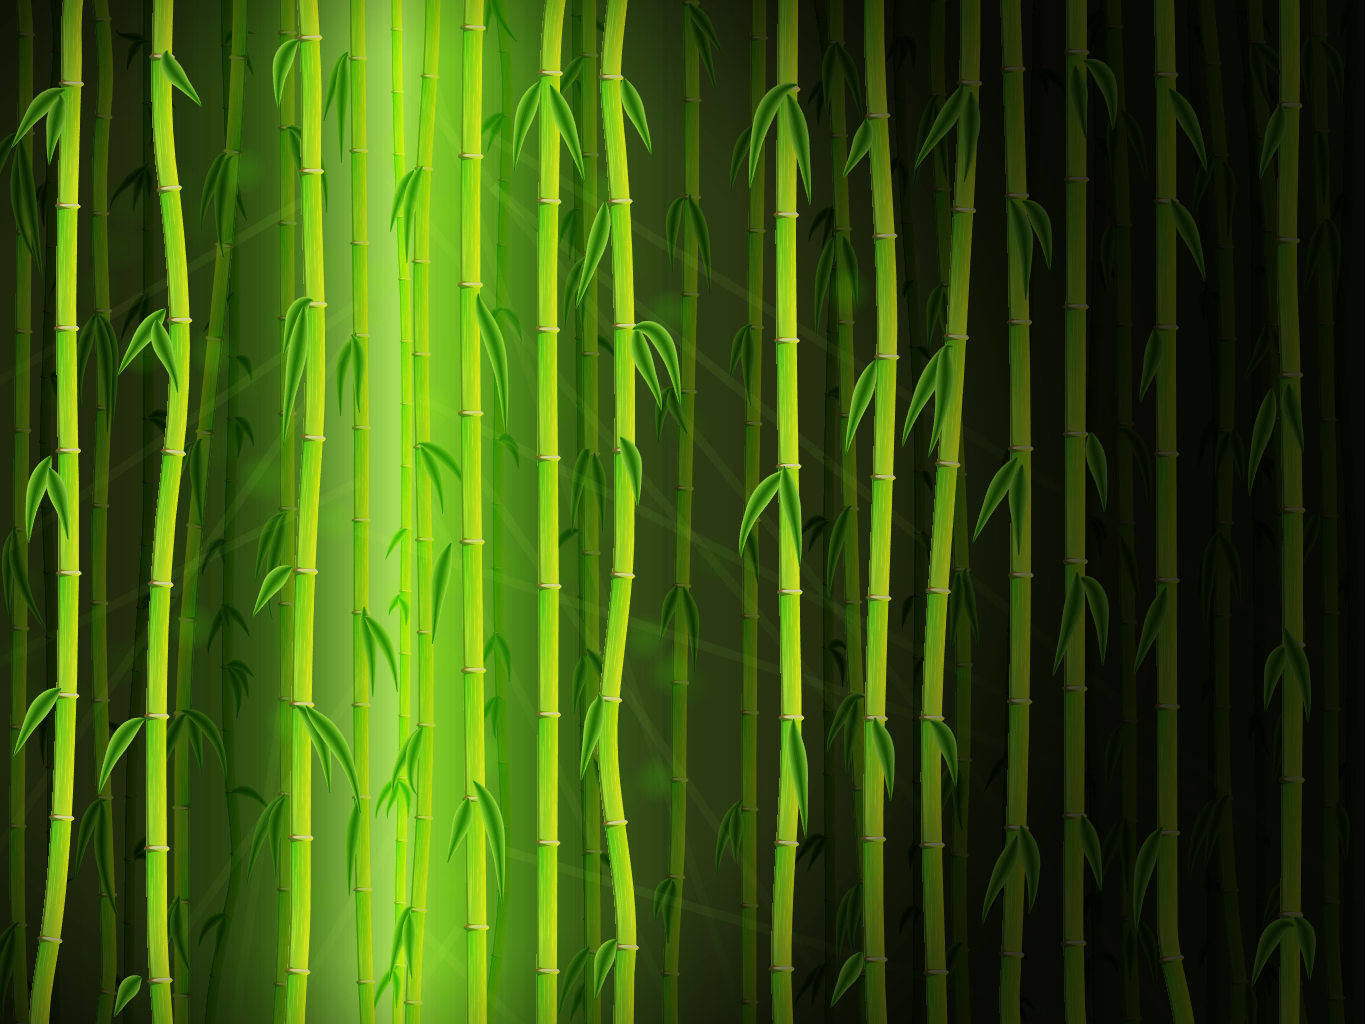
\includegraphics[height=1.4in] {benchmarks/images/fig_bamboo.png}
   \label{fig:bamboo}
 }
 %\qquad
 \\%
 \subfigure[archerfish.ai]{
   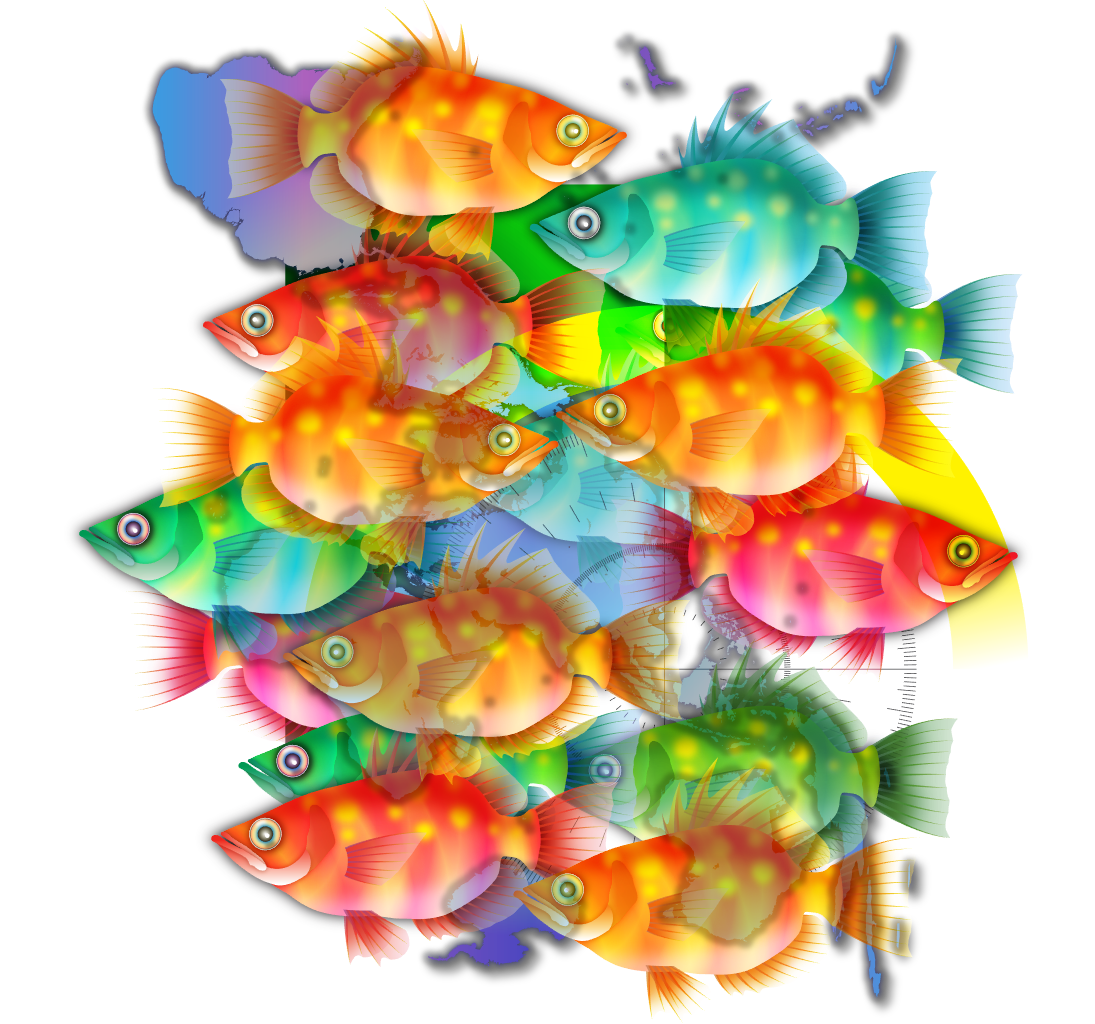
\includegraphics[height=1.62in] {benchmarks/images/fig_archerfish.png}
   \label{fig:archerfish}
 }
 \qquad
 \subfigure[Blue Mirror.ai]{
   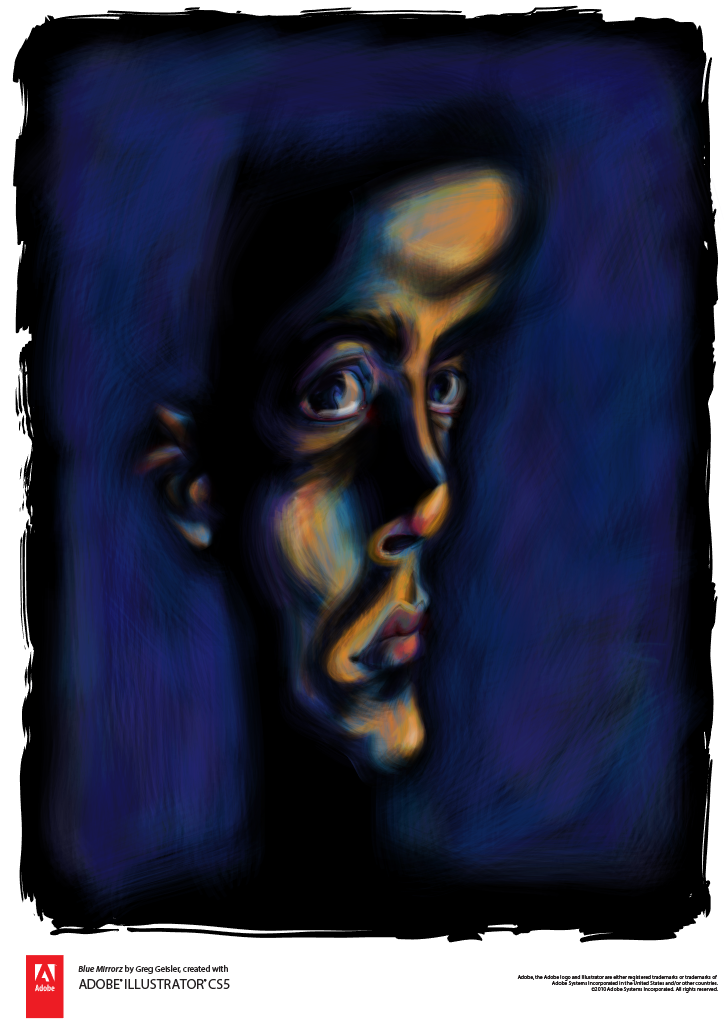
\includegraphics[height=1.62in] {benchmarks/images/fig_blue_mirror.png}
   \label{fig:blue-mirror}
 }\\%
 \subfigure[whale2.ai]{
   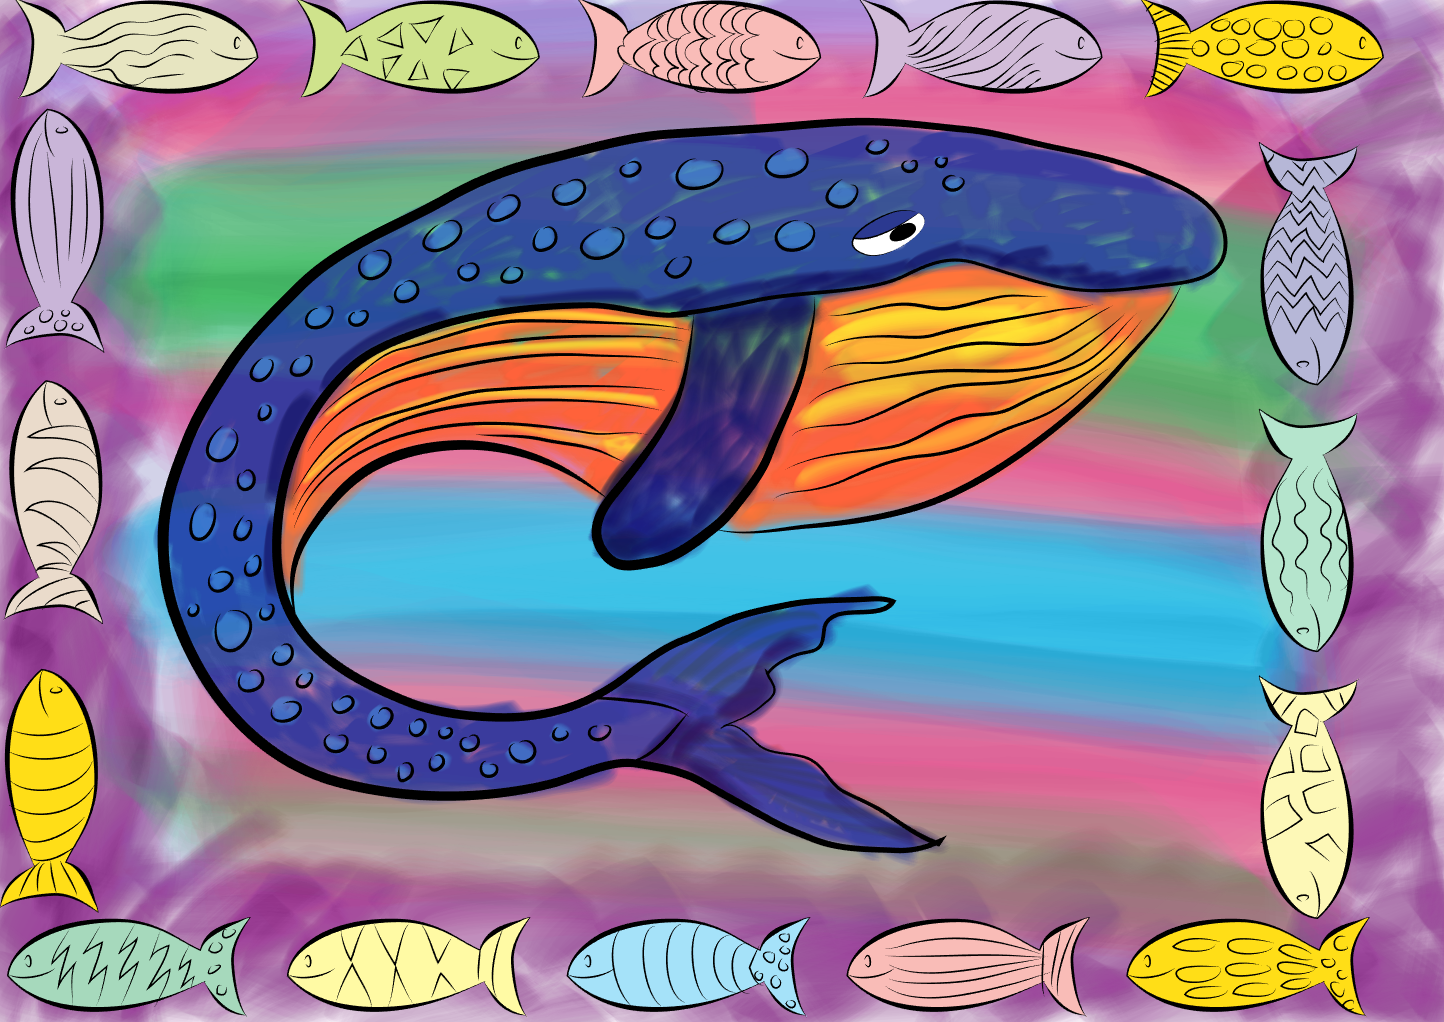
\includegraphics[height=1.4in] {benchmarks/images/fig_whale.png}
   \label{fig:whale}
 }
 \\
 %\subfigure[Beer-Glass.ai]{
 %  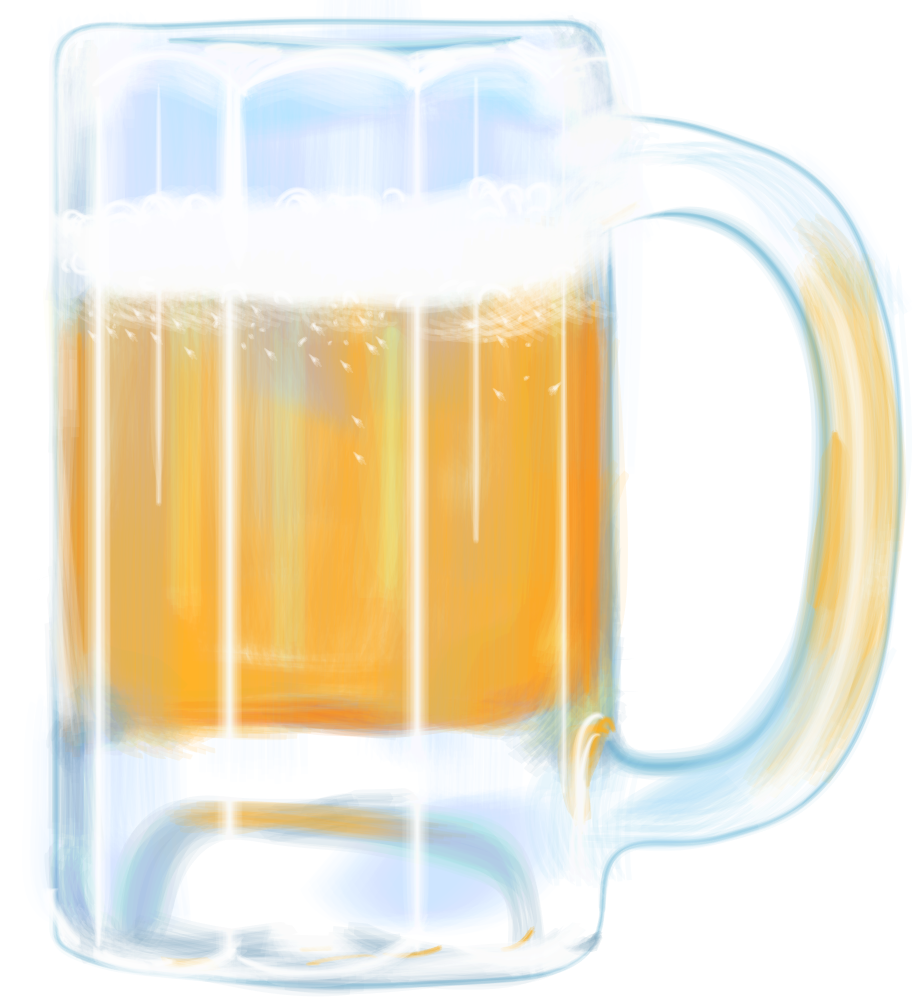
\includegraphics[width=1.2in] {benchmarks/images/fig_beer_glass.png}
 %  \label{fig:beer-glass}
 %}\qquad%
 %\subfigure[Carrot Tree Restaurant.ai]{
 %  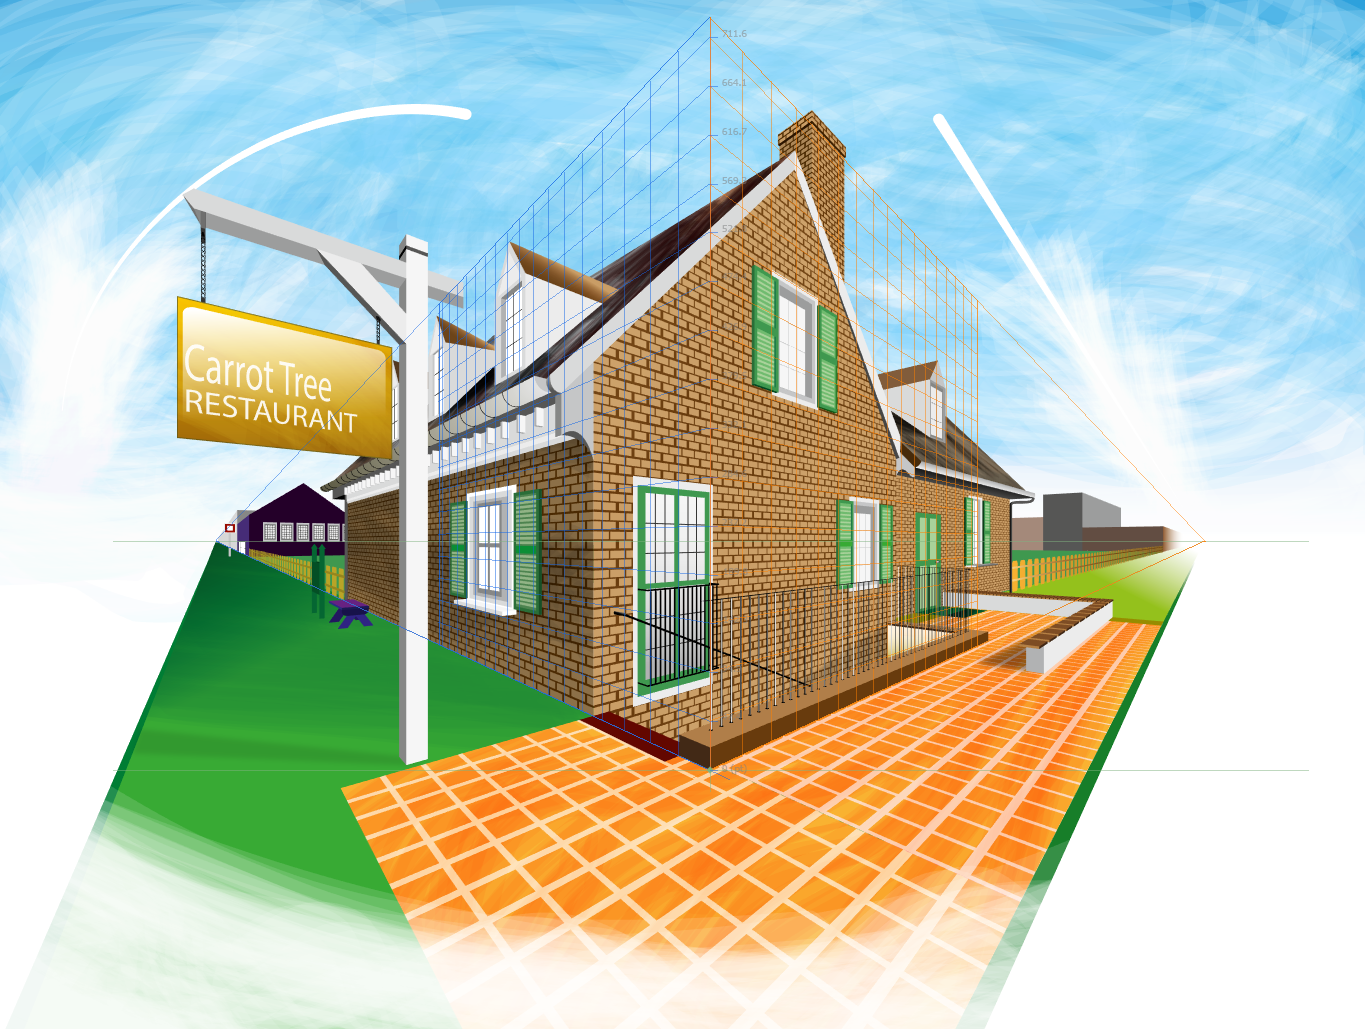
\includegraphics[width=1.6in] {benchmarks/images/fig_carrot_tree.png}
 %  \label{fig:carrot-tree}
 %}\\%
 %\subfigure[Crowd (1).ai]{
 %  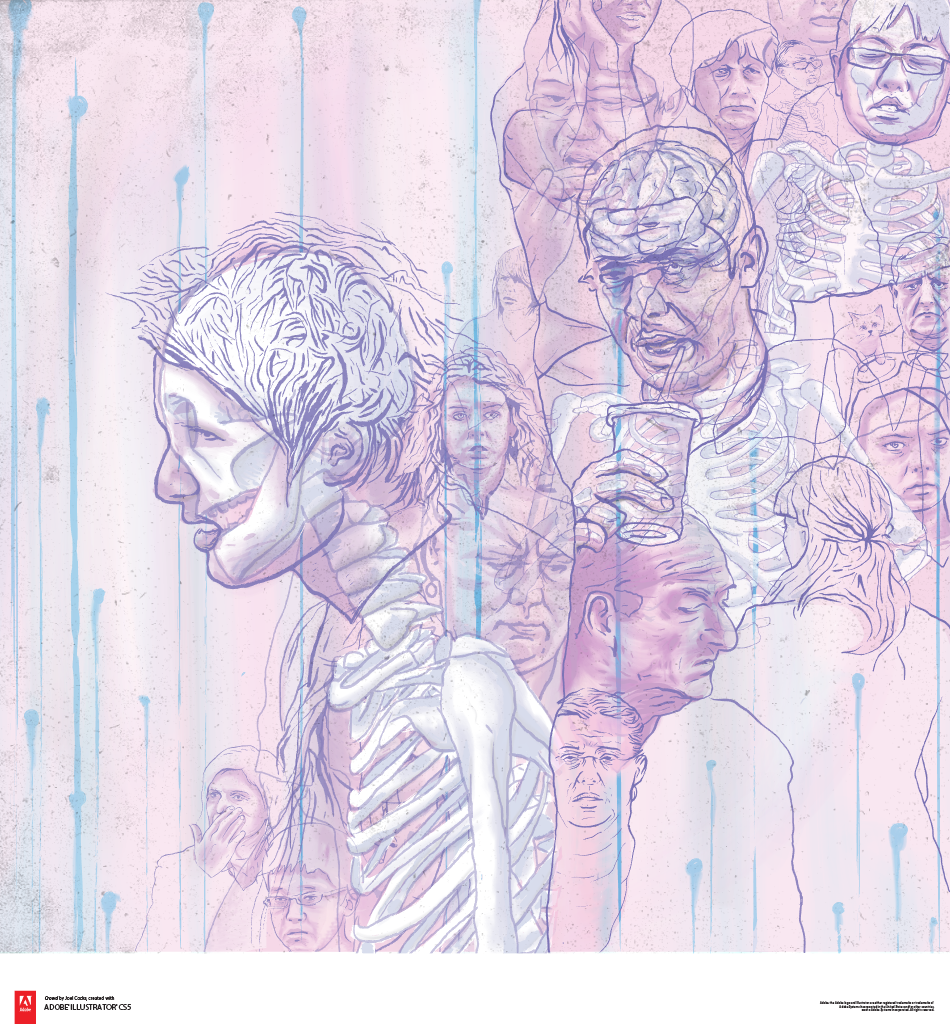
\includegraphics[width=1.1in] {benchmarks/images/fig_crowd.png}
 %  \label{fig:crowd}
 %}\qquad%
 \subfigure[Tropical Reef.ai]{
   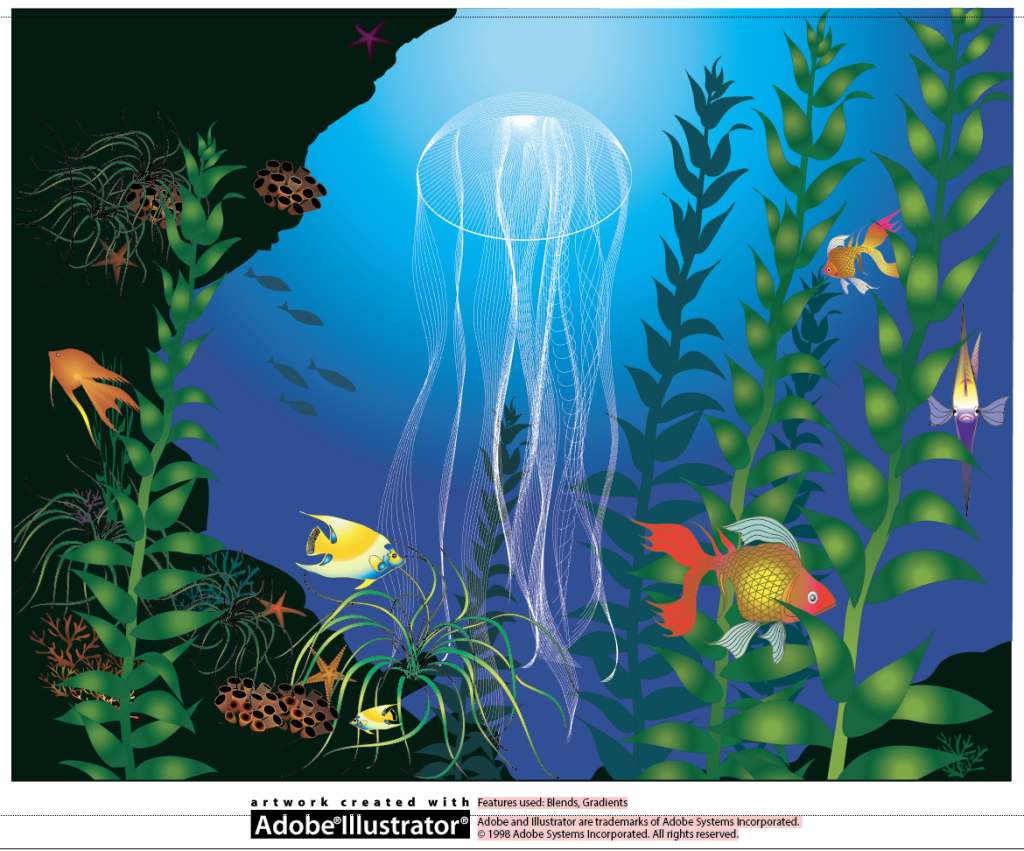
\includegraphics[height=1.4in] {benchmarks/images/ai_tropical_reef.png}
   \label{fig:reef}
 }
 \\
 %\qquad%
 \subfigure[bigBlend2.ai]{
   
\includegraphics[height=1.4in] {benchmarks/images/fig_big_blend.png}
   \label{fig:big-blend}
 }
\caption{Challenging \Illustrator/ artwork for benchmarking.}
\label{fig:scenes}
\end{figure}


\subsection{Benchmarking RGB Artwork}

Table \ref{table:rgb-scene-performance} presents our benchmarking results
for RGB color model rendering.
Our benchmarking method executes a script that zooms and pans over
the content to mimic the kind of fast view changes an artist would use
during interactive inspection of the artwork.  During the benchmark,
the \Illustrator/ application and document view are both {\em maximized}
for the most visible pixels.


Our system configuration is a Windows 7 PC with a Xeon E3-1240 V2
CPU @ 3.40GHz (4 cores), 8 GB RAM, and NVIDIA GeForce GTX 780 Ti GPU.
\AGM/'s CPU-based renderer automatically takes advantages of the CPU's
multiple cores for parallel rendering.  NVIDIA's OpenGL driver is
automatically configured for dual-core operation so the application
thread communicates OpenGL commands to a driver thread so application
and driver processing operate concurrently.  We benchmarked the 64-bit
version of the latest \Illustrator/.
\Illustrator/ always renders with 8x multisampling.


We are particularly interested in how GPU-accelerated \Illustrator/
can improve the user experience in expectation of the mass-market
adoption of {\em 4K resolution} displays so we report frame times
using Full HD resolution (1920x1080) and Ultra HD (3840x2160) monitors.
Increasing the display resolution from Full to Ultra HD increases the
geometric mean of the relative increase in CPU render time by 190\%;
but only 22\% for the GPU-accelerated transition.  We note that the
CPU rendered Ultra HD frame render times are on the order of seconds;
the GPU-accelerated frame rates are 5+ frames per second (7.9 average)
so still within what artists tolerate as interactive.

%%%% OLD TABLE
%
%\begin{table}
%    \begin{tabular}{| l | c || r | r | r |}
%    \hline
%      & Monitor HD    &        &        & \\
%Scene & Resolution & CPU ms & GPU ms & Gain \\ \hline \hline
%
%\hyperref[fig:bamboo]{WF\_Bamboo}	&	Full 	&	320	&	164	&	2.1x \\ % native CMYK
%\hspace{0.3em} \hyperref[fig:bamboo]{Scene}	&	Ultra	&	1013	&	178	&	5.6x \\ \hline
%
%\hyperref[fig:archerfish]{ArcherFish}	&	Full 	&	193	&	65	&	2.8x \\ % native RGB
%	&	Ultra	&	645	&	79	&	6.6x \\ \hline
%
%\hyperref[fig:whale]{whale2}	&	Full &	341	&	110	&	3.5x \\  % native RGB
%	&	Ultra	&	906	&	121	&	7.1x \\ \hline
%
%\hyperref[fig:blue-mirror]{BlueMirror}	&	Full &	923	&	193	&	4.2x \\  % native RGB
%	&	Ultra	&	2011	&	212	&	7.8x \\ \hline
%
%\hyperref[fig:beer-glass]{Beer-Glass}	&	Full 	&	229	&	46	&	5.3x \\  % native CMYK
%	&	Ultra	&	588	&	66	&	9.9x \\ \hline
%
%\hyperref[fig:carrot-tree]{Carrot Tree} 	&	Full 	&	130	&	35	&	3.5x \\  % native CMYK
%\hspace{0.3em} \hyperref[fig:carrot-tree]{Restaurant} &	Ultra	&	420	&	47	&	9.3x \\ \hline
%
%\hyperref[fig:crowd]{Crowd (1)} 	&	Full 	&	712	&	150	&	4.8x \\  % native CMYK
%	&	Ultra	&	1963	&	203	&	10.0x \\ \hline
%
%\hyperref[fig:big-blend]{bigblend2} 	&	Full 	&	656	&	94	&	6.2x \\  % native CMYK
%	&	Ultra	&	2361	&	109	&	16.7x \\ \hline
%
%    \hline
%    \end{tabular}
%
%\caption{Average frame time in milliseconds rendering complex art scenes at varying zooms and panning, comparing the
%existing CPU rendering mode to our new GPU-accelerated mode.  {\em Gain} is the geometric mean of the speedup of
%GPU over the CPU mode for corresponding benchmark frames.
%}
%\label{table:rgb-scene-performance}
%
%\end{table}

\begin{table}
    \begin{tabular}{| l | c || r | r | r |}
    \hline
RGB mode & Monitor HD    &        &        & \\
Scene & Resolution & CPU ms & GPU ms & Gain \\ \hline \hline

\hyperref[fig:bamboo]{WF\_Bamboo}	&	Full 	&  320	&	174	&	3.53x \\ % native CMYK
\hspace{0.3em} \hyperref[fig:bamboo]{Scene}	&	Ultra	&1071	&	219	&	5.23x	\\ \hline

%\hyperref[fig:carrot-tree]{Carrot Tree} 	&	Full 	&104	&	22	&	4.54x	\\  % native CMYK
%\hspace{0.3em} \hyperref[fig:carrot-tree]{Restaurant} &	Ultra	&292	&	38	&	7.49x	\\ \hline

\hyperref[fig:whale]{whale2}	&	Full &336	&	37	&	8.41x	\\  % native RGB
	&	Ultra	&1015	&	129	&	8.02x	\\ \hline

\hyperref[fig:archerfish]{ArcherFish}	&	Full 	&259	&	28	&	9.04x	\\ % native RGB
	&	Ultra	&979	&	100	&	9.59x	\\ \hline

%\hyperref[fig:beer-glass]{Beer-Glass}	&	Full 	&291	&	24	&	9.29x	\\  % native CMYK
%	&	Ultra	&562	&	80	&	7.38x	\\ \hline

\hyperref[fig:reef]{Tropical Reef}	&	Full 	&64	&	20	&	3.36x	\\  % native CMYK
	&	Ultra	&179	&	30	&	6.28x	\\ \hline

\hyperref[fig:blue-mirror]{BlueMirror}	&	Full &1209	&	100	&	11.39x	\\  % native RGB
	&	Ultra	&2971	&	279	&	10.98x	\\ \hline

%\hyperref[fig:crowd]{Crowd (1)} 	&	Full 	&636	&	49	&	14.31x	\\  % native CMYK
%	&	Ultra	&1875	&	149	&	14.43x	\\ \hline

\hyperref[fig:big-blend]{bigblend2} 	&	Full 	&828	&	44	&	14.38x	\\  % native CMYK
	&	Ultra	&3211	&	142	&	17.54x	\\ \hline

    \hline
    \end{tabular}

\caption{Average frame time in milliseconds rendering complex art
scenes in RGB document mode (CMYK artwork is forced to RGB) at varying
zooms and panning, comparing the existing CPU rendering mode to our new
GPU-accelerated mode.  {\em Gain} is the geometric mean of the speedup
of GPU over the CPU mode for corresponding benchmark frames.
}
\label{table:rgb-scene-performance}

\end{table}

\begin{table}
    \begin{tabular}{| l | c || r | r | r |}
    \hline
CMYK mode & Monitor HD    &        &        & \\
Scene & Resolution & CPU ms & GPU ms & Gain \\ \hline \hline

\hyperref[fig:bamboo]{WF\_Bamboo}	&	Full 	&  392	&	405	&	1.34x \\ % native CMYK
\hspace{0.3em} \hyperref[fig:bamboo]{Scene}	&	Ultra	&1520	&	630	&	2.37x	\\ \hline

\hyperref[fig:reef]{Tropical Reef}	&	Full 	&99	&	22	&	4.80	\\  % native CMYK
	&	Ultra	&311	&	38	&	9.28x	\\ \hline

\hyperref[fig:big-blend]{bigblend2} 	&	Full 	&861	&	111	&	6.73x	\\  % native CMYK
	&	Ultra	&3542	&	381	&	10.55x	\\ \hline

    \hline
    \end{tabular}

\caption{Average frame time in milliseconds rendering complex CMYK art
scenes at varying
zooms and panning, comparing the existing CPU rendering mode to our new
GPU-accelerated mode.  {\em Gain} is the geometric mean of the speedup
of GPU over the CPU mode for corresponding benchmark frames.
}
\label{table:cmyk-scene-performance}

\end{table}

\subsection{Benchmarking CMYK Artwork}

Table~\ref{table:cmyk-scene-performance} presents CMYK benchmarking results for the three ``native CMYK'' scenes
listed in Table~\ref{table:scene-metrics}.
Whereas the benchmarking of these scenes in Table~\ref{table:rgb-scene-performance} forced the scenes
be converted to RGB, Table~\ref{table:cmyk-scene-performance} benchmarks these scenes in their
native CMYK color space by rendering with a CMYK framebuffer.

The WF\_BambooScene scene is included specifically because it demonstrates rather poor GPU rendering performance,
particularly when rendered in the scene's native CMYK color space.
The WF\_BambooScene scene is an example of a scene constructed in ways that stress GPU rendering with poor results---though the scene is quite challenging for CPU rendering too!
First the scene itself has a large number of paths,
a variety of blend modes, and uses knockout.  The scene already has a large number of transparency groups, but many become
non-trivial groups when used with non-{\em Normal} blend modes and knock-out.
Recall \NVbea/ limitations that make blend modes overly expensive in CMYK rendering (Section \ref{sec:tweaks}).
Additionally when zoomed out of the scene, there is a large number of intricate
paths placed invisibly outside the scene's framed view (this is not uncommon for artists to do as
a way of stashing fragments of artwork).  The effect is acceptable GPU-acceleration when zoomed into
the CMYK scene but worse-than-CPU-rendering performance when zoomed out.  Performance is good zoomed
in because the pathological features of the scene get view culled away.

\begin{figure}[tb]
  \center{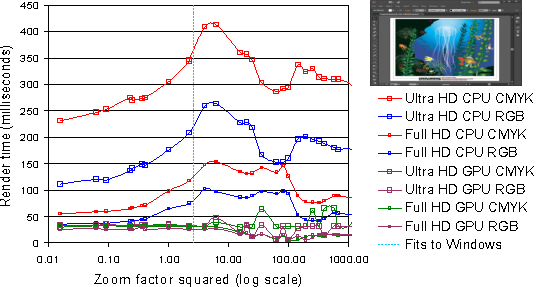
\includegraphics[width=\columnwidth]{images/illustrator_performance.pdf}}
  \caption{\label{fig:zoom-perf}
Rendering time for Tropical Reef.ai scene, comparing GPU vs. CPU, Full vs. Ultra HD, and RGB vs. CMYK at over a large range of zoom factors squared.  Dashed vertical lines indicate the zoom factor when the scene ``Fits to Window'' for Full and Ultra HD respectively.
}
\end{figure}

We now look at a more typical scene in detail.
Figure~\ref{fig:zoom-perf} graphs the render time for at a variety of zoom levels
for the (native CMYK) Tropical Reef scene.  Illustrator documents are in ``real world''
dimensions so a 100\% zoom corresponds to its printed dimensions.  We graph the zoom factor squared
(so 1 is a 100\% zoom and 4 is a 200\% zoom) because this normalizes the screen-space area of a given scene region.
The graph shows the scene rendered in
all eight combinations of CPU/GPU rendering, Full/Ultra HD resolution, and CMYK/RGB color models
over a range of zoom levels.  While the original scene is authored in CMYK, by forcing a conversion
to the RGB color mode, we can compare the relative expense of CMYK relative to RGB rendering.

While the window size in pixels is constant at either Full or Ultra
HD resolution, the render time is not stable at increasing zoom levels
because many objects can be culled from the scene as the zoom increases
while also small objects become large and hence more expensive to draw.
This factor affects both the CPU and GPU render times but in different
ways we now explore.

The CPU renderer is sensitive to having a large number of objects, and
hence active edges, to process.  Also complex shading and blending is
relatively more expensive for the CPU while shading and blending are
quite efficient for the GPU.  In contrast while the CPU's scan-line 
rasterizer is quite work-efficient and ``cache friendly'' because it operates
on just a scan-line at a time, the GPU renderer is challenged when
paths are large in screen space so the overdraw from the ``stencil'' step
becomes rasterization bound.  Lots of stencil counting that ultimately cancels to zero or
generates large winding number magnitudes create costly rasterization burdens for the GPU.
Likewise expensive quadratic discard shaders for curved stroked segments become
expensive when the stroke width is more than a fix pixels wide in screen space.

Even so, GPU performance is consistently faster than the CPU performance but subject
to more significant variations at different zoom levels.  To help quantify the relative
cost of CMYK rendering via the GPU we can compare native CMYK rendering on the GPU to
an RGB-converted version of the Tropical Reef content in Figure~\ref{fig:zoom-perf}.
RGB-converted rendering averages
36\% (Full HD) to 43\% (Ultra HD) faster than CMYK rendering with the CPU.
The GPU averages 6\% (Full HD) to 9\% (Ultra HD) faster when the
CMYK artwork is converted to RGB but these averages mask significant
variability.  So while the framebuffer memory consumption for CMYK is at least double
the storage for RGB color mode rendering, the observed performance cost is not nearly so bad
and is still much faster than CMYK rendering on the CPU.

\subsection{Comparison with Recent Work}
\label{sec:mpvg}

\cite{GanEtAl14} provides performance results for a number of SVG scenes
using a massively-parallel vector graphics (MPVG) system based on CUDA.  Table~\ref{table:mpvg}
presents a subset of their scenes most relevant to an Illustrator artist with results from our comparable PC configuration.  Our rendering performance relies on
\NVpr/ but performs markedly better than the \NVpr/ performance reported in their paper.
We attribute this to forcing use of NVIDIA's dual-core
driver and Illustrator's tuned OpenGL usage and scene traversal.
For all but two of scenes in our table, GPU-accelerated Illustrator is faster than their published results---the
exceptions are a detailed but inefficiently authored (so CPU bound) Paris map and their---arguably pathological---Contour scene.

MPVG's strengths are antialiasing quality and an ability to handle what would typically be considered
inefficiently structured scenes---strengths we readily acknowledge.
Since Illustrator supports just 8x multisampling and their reported
image resolutions are rather low, we provide ``double resolution''
rendering results as an alternative for their 32x rendering quality.

While MPVG's rendering quality and novelty of approach is impressive,
Illustrator must support the entire PDF rendering model including CMYK, blend modes,
transparency groups, etc. all while making everything editable.

\begin{table}
    \begin{tabular}{| l | l || r | r | r |}
    \hline
      &            & MPVG & MPVG & Illustrator \\
Input & Resolution & 8x & 32x & GPU 8x \\
    \hline
    \hline

Car & 1024x682 & 12.86 & 14.73 & 2.94 \\
    & 2048x1364 & & & 3.09
\\ \hline
Drops & 1024x1143 &14.28 & 18.59 & 2.29 \\
    & 2048x2286 & & & 6.21
\\ \hline
Embrace & 1024x1096 &15.50 & 19.38 &  1.69 \\
    & 2048x2192 & & & 3.63
\\ \hline
Reschart & 1024x625 &8.51 & 11.14 & 1.92 \\
    & 2048x1250 & & & 2.60
\\ \hline
Tiger & 1024x1055 &12.89 & 17.24 &  1.48 \\
    & 2048x2110 & & & 5.34
\\ \hline
Boston & 1024x917 &37.22 & 41.81 &  2.66 \\
    & 2048x1834 & & & 5.02
\\ \hline
Hawaii & 1024x844 &26.16  &29.48 &  3.83 \\
    & 2048x1688 & & & 8.75
\\ \hline
Contour & 1024x1024 &30.07 & 30.36 & 90.53 \\
    & 2048x2048 & & & 328.57
\\ \hline
Paris 50K & 1024x1024 &26.82 & 25.22 & 65.53 \\
    & 2048x2048 & & & 64.23
\\ \hline

    \end{tabular}
    \caption{Comparison of SVG content render times (in milliseconds) reported by \protect\cite{GanEtAl14} to our work with Illustrator.}
\label{table:mpvg}

\end{table}


% !TEX root = illustrator_submission.tex

\section{Conclusions}
\label{sec:conclusion}

We have succeeded in GPU-accelerating \Illustrator/ despite
decades of being unadvantaged by graphics hardware.  Our
benchmarking shows significant speed-ups, particularly at 4K resolution.
Our contributions introduce novel techniques for supporting CMYK color
space rendering on existing GPUs, proper transparency group support
including non-isolated groups and knock-out, and mapping PDF's gradient
mesh shading to GPU tessellation.

\subsection{Broader Hardware Support}
\label{sec:standardization}

OpenGL 4.4 is the multi-vendor standard baseline for our GPU-acceleration
effort but \Illustrator/ also requires the \NVpr/ and \KHRbea/
extensions.  As a practical matter, today just NVIDIA GPUs (Fermi
generation \cite{Fermi} and beyond) on Windows support the prerequisite
OpenGL functionality.  \Illustrator/ supports a wide range
of system configurations so we
naturally want these GPU-acceleration benefits supported more broadly.
We are exploring ways to support a broader range of GPUs.
Standardization of \NVpr/ would make this much easier.

\ifdefined\NOSHOW
We happily note all the blend mode functionality we need
is now standardized as \KHRbea/ \cite{KHRbeaSpec} though other shader-based
alternatives (see Section \ref{sec:blendalternatives}) to implement blend modes are worth investigating.
\fi

\subsection{Future Work}
\label{sec:futurework}

Much of the user interface of \Illustrator/ today assumes
re-rendering the scene is slow and expensive.  For example, the
user interface encourages users to {\em isolate} a portion of the
scene to avoid rendering the complete scene.  Similarly editing
often happens by dragging overlaid ``blue lines'' rather than a more
{\em what-you-see-is-what-you-get} interaction model.  We hope the
GPU-acceleration we have introduced into \Illustrator/ will facilitate
more powerful, intuitive, and fluid user interfaces for vector graphics
editing.

We note a number of inspired research efforts relevant to vector
graphics editing that are either conceived with GPU-acceleration
in mind---such as diffusion curves \cite{Andronikos2013}---or
introduce vector graphics complexity that overwhelms conventional
CPU-based vector graphics rendering---such as digital micrography
\cite{Maharik:2011:DM:2010324.1964995}.  We hope by bringing
\Illustrator/ to the GPU, these techniques will become tractable to
support within \Illustrator/ and thereby be adopted by digital artists.

Our framebuffer memory usage is substantial.  We want to incorporate
NVIDIA's \NVfms/ OpenGL
extension \cite{FramebufferMixedSamples}
that allows an OpenGL framebuffer object to have fewer color
samples than stencil samples (and no depth samples) to reduce memory usage without reducing
the rasterization quality of path rendering.  

We believe graphics hardware architects can improve the support for
print-oriented features---in particular the CMYK color space.  Doing so
would greatly reduce the memory bandwidth, memory footprint, and greatly
simplify the complex orchestration of multiple RGBA color buffers required
to accomplish CMYK rendering.

\ifreviewelse
{}
{
\section*{Acknowledgments}

We thank:
David Aronson,
Rui Bastros,
Jeff Bolz,
Rajesh Budhiraja,
Nathan Carr,
Qingqing Deng,
Vineet Punjabi,
E Ramalingam,
Anubhav Rohatgi,
Lekhraj Sharma,
Gopinath Srinivasan,
Tarun Beri,
and our anonymous reviewers.
}


\pdfbookmark[1]{References}{bkmk:references}
\bibliographystyle{acmsiggraph}
%\nocite{*}  % include references not cited in the paper
\bibliography{path_rendering}

\end{document}
